% NeurIPS 2026 workshop paper.
% Requires neurips_2026.sty in this directory (official kit, revised January 2026).
% Build:  pdflatex context_fatigue.tex   (x2 for refs)
%
% Track option: `dblblindworkshop` anonymises the author block and adds line numbers.
% For a single-blind workshop swap it for `sglblindworkshop`; add `final` alongside
% either one for the camera-ready.

\documentclass{article}

\usepackage[dblblindworkshop]{neurips_2026}

\usepackage[utf8]{inputenc}
\usepackage[T1]{fontenc}
\usepackage[hidelinks]{hyperref}
\usepackage{url}
\usepackage{booktabs}
\usepackage{amsmath}
\usepackage{amssymb}
\usepackage{microtype}
\usepackage{enumitem}
\usepackage{caption}
\usepackage{subcaption}
\usepackage{graphicx}
\usepackage{float}
\usepackage{tikz}

% compaction for a workshop paper
\setlength{\textfloatsep}{5pt plus 2pt minus 2pt}
\setlength{\intextsep}{5pt plus 2pt minus 2pt}
\captionsetup{skip=2pt}
\captionsetup[sub]{skip=1pt}
\setlist[itemize]{nosep,leftmargin=1.4em,topsep=2pt}

\title{Breaking Down Context Rot in LLMs}

% REQUIRED for the workshop track: the footnote on page 1 reads "Workshop: <this>."
\workshoptitle{Interpretability as a Science}

% Repository link follows the style's anonymity flag: anonymized under [dblblindworkshop],
% real under [sglblindworkshop], [final], [preprint], or [nonanonymous].
\makeatletter
\if@anonymous
  \newcommand{\repourl}{https://anonymous.4open.science/r/Breaking-Down-Context-Rot-A553/}
\else
  \newcommand{\repourl}{https://github.com/Ronen09/Breaking-Down-Context-Rot}
\fi
\makeatother

\author{%
  Ronen Raj Roy\\
  \texttt{ronex665@gmail.com}\\
}

\begin{document}

\maketitle

\begin{abstract}
Long conversations are said to wear language models down, but standard evaluations confound
accumulation (more context) with dilution (the answer-bearing tokens becoming a smaller, more
distant, more contested fraction of it). We separate them in streams of localized tasks,
each answerable from its own question, where accumulation grows the context without diluting
anything the current answer needs and a span-attention clamp sets any span's attention share
directly. All experiments run on OLMo-2-7B-Instruct.

Accumulation alone costs \textbf{nothing}: accuracy and instruction adherence stay flat to
$90\%$ fill, with declines larger than $2.9$ and $5.5$ points excluded at $95\%$. That null is the
paper's starting point: three other things in a growing context do cost, and length is only
the usual way of causing them at once. Displacement, moving a task's
evidence back into the context, costs accuracy, and removing the evidence's attention mass
with nothing else moved reproduces the full penalty, smoothly and without a threshold.
Competition, near-duplicate context, costs a further $8.5$ points while the evidence's
attention barely moves; closing every context mention of the answer options recovers
\textbf{56\%} against a random-closure control at zero, placing the cost on the competitors
rather than the evidence. Precedent, filler that demonstrates an applicable answer
shape, erodes an instructed output format completely ($0.875\to0.000$ within three filler
turns, accuracy unharmed) while the instruction's attention holds and its content stays
linearly decodable.

The same closure that rescues competition restores nothing for precedent---competition is
generation-time reading, while the precedent mode is set at prefill, its carrier localized to
the chat template's delimiter tokens in the lower half of the stack. All of it
replicates on Qwen2.5-7B-Instruct except competition (penalty gone, attention signature
inverted) and the erosion (staged, not total). Context rot in localized streams is
displacement, competition, and precedent, and only the first is attention dilution proper.
\end{abstract}

\section{Introduction}
\label{sec:intro}

A recurring worry about long conversations is context rot: as turns accumulate, the model
is said to degrade. The phenomenology is real. On a repeating multiple-choice task,
instruction-tuned models grow more confident as context fills: next-token entropy
drops roughly $3$--$4\times$ on Qwen-2.5-7B \citep{qwen2025} and Llama-3.1-8B
\citep{llama3herd}. On OLMo-2-Instruct the last token's attention leaves
the system prompt (correlation with fill $-0.93$) and the current query ($-0.71$) for the most
recent prior cases ($+0.89$), all monotone.

One reading attributes the degradation to length itself. Long context comes in two shapes,
and they present different problems. In the first, one task spans the whole context: a
long document, a buried needle, a growing codebase. Length there mechanically dilutes
the answer-bearing tokens among irrelevant ones, and a measured degradation conflates the cost
of accumulation with the cost of the target being harder to attend to (``lost in the middle,''
\citealp{liu2023lost}). In the second, the context is a stream of localized tasks, each
self-contained and already finished: an agent transcript of locally-scoped steps, a session of
independent questions. Accumulation there grows the context without diluting anything the
current answer needs. The context-rot literature measures the first shape almost exclusively, where the two costs
cannot be separated. This paper measures the second, where they can and where the two accounts
predict opposite outcomes (Appendix~\ref{app:related}). Retrieval is the case between them, a
localized stream whose current answer depends on evidence sitting back in the context, and
\S\ref{sec:displacement} builds it by moving the evidence back.

We separate the candidate causes inside one harness (Fig.~\ref{fig:framework}) and ask three
questions. \textbf{RQ1}: does accumulation alone, with the evidence for every answer held at
the current query, degrade accuracy or instruction adherence? \textbf{RQ2}: when dilution does
cost accuracy, is the cost mediated by the evidence's attention mass? We split dilution into
its two components, the evidence becoming distant and the context becoming
confusable, and test each causally. \textbf{RQ3}: if adherence survives context fill,
what erodes instruction-following under accumulation?

RQ3 takes up \citet{dongre2026attentioncloses}, who showed that attention to the system prompt
closes over accumulated filler and asked whether behavior survives that closure, finding the
answer architecture-indexed. Our precedent arms answer with a graded instrument on one
architecture.

Accumulation is the design's null arm (RQ1). Our contributions are the harness and one causal
result for each mechanism that costs something:

\begin{itemize}
  \item A harness that makes accumulation and dilution independent, by accumulating individually
        localized tasks whose evidence never moves, and a span-attention clamp that sets
        any span's post-softmax share with a bit-identical no-op at scale $1$
        (\S\ref{sec:method}).
  \item \textbf{Displacement}, the retrieval case built inside the stream, is causally
        sufficient: removing the evidence's attention mass with
        nothing moved reproduces the penalty in full, and the mass$\to$accuracy
        relationship is smooth and graded with no threshold in it (RQ2, \S\ref{sec:displacement}).
  \item \textbf{Competition} is a second mechanism, costing accuracy at
        constant evidence mass. Closing the competitor mentions recovers $56\%$ of
        the penalty; both accuracy mechanisms are attentional, on different spans, and
        span-targeted closure tells them apart (RQ2, \S\ref{sec:competition}).
  \item \textbf{Precedent} costs compliance rather than accuracy. Accumulated demonstrations
        erode an instructed format only when their shape transfers to the probe, immediately and
        with accuracy unharmed. The erosion is not carried by the instruction's attention, yet
        re-weighting or re-presenting the instruction each fully reverse it
        (RQ3, \S\ref{sec:precedent}--\S\ref{sec:mode}).
\end{itemize}

\begin{figure}[t]
  \centering
  \begin{tikzpicture}[xscale=1.06, yscale=0.47, every node/.style={font=\scriptsize}]
    % row template lengths: sys 0-1.3, filler 1.4-7.0 (4 boxes), probe 7.2-9.0
    \newcommand{\strip}[1]{
      \draw[fill=green!14] (0,#1) rectangle (1.3,#1+0.7);
      \node at (0.65,#1+0.35) {system};
      \foreach \i in {0,...,3} {
        \draw[fill=black!7] (1.4+\i*1.45,#1) rectangle (2.75+\i*1.45,#1+0.7);
      }
      \draw[fill=blue!14] (7.2,#1) rectangle (9.0,#1+0.7);
      \node at (8.1,#1+0.35) {current question};
    }
    % Row 1: accumulation
    \strip{6.6}
    \foreach \i in {0,...,3} { \node at (2.075+\i*1.45,6.95) {case \pgfmathparse{int(\i+1)}\pgfmathresult}; }
    \filldraw[blue!70!black] (8.62,6.78) circle (0.06);
    \node[right,font=\footnotesize] at (9.15,7.25) {\textbf{1. Accumulate} (RQ1)};
    \node[anchor=north west,text width=3.9cm,font=\footnotesize] at (9.15,6.95) {grow the filler. The evidence ({\color{blue!70!black}$\bullet$}) stays at the query};
    \node at (5.0,6.28) {$+\;\cdots$ more finished cases};
    % Row 2: displacement
    \strip{4.4}
    \filldraw[blue!70!black] (3.4,4.58) circle (0.06);
    \draw[->,dashed,blue!70!black] (8.1,5.14) to[bend right=14] (3.4,5.14);
    \node[right,font=\footnotesize] at (9.15,5.05) {\textbf{2. Displace} (RQ2a)};
    \node[anchor=north west,text width=3.9cm,font=\footnotesize] at (9.15,4.75) {move the evidence $k$ turns back. Fill and items fixed};
    % Row 3: competition
    \strip{2.2}
    \foreach \i in {0,...,3} {
      \draw[fill=red!14] (1.4+\i*1.45,2.2) rectangle (2.75+\i*1.45,2.9);
      \node at (2.075+\i*1.45,2.55) {near-dup};
    }
    \filldraw[blue!70!black] (8.62,2.38) circle (0.06);
    \node[right,font=\footnotesize] at (9.15,2.85) {\textbf{3. Compete} (RQ2b)};
    \node[anchor=north west,text width=3.9cm,font=\footnotesize] at (9.15,2.55) {make the filler confusable. Distance $0$, fill fixed};
    % Row 4: precedent
    \strip{0.0}
    \draw[very thick,green!45!black] (0,0) rectangle (1.3,0.7);
    \foreach \i in {0,...,3} {
      \draw[fill=red!22] (2.28+\i*1.45,0.06) rectangle (2.69+\i*1.45,0.64);
    }
    \node at (5.0,-0.35) {\color{red!60!black}demonstrated answer shape};
    \node[right,font=\footnotesize] at (9.15,0.65) {\textbf{4. Demonstrate} (RQ3)};
    \node[anchor=north west,text width=3.9cm,font=\footnotesize] at (9.15,0.35) {let the filler's replies demonstrate an answer shape};
  \end{tikzpicture}
  \caption{\textbf{The localized-stream framework: four independent knobs on one transcript.}
  Each stream accumulates self-contained cases, so the evidence for the current answer sits at
  the current question by default and every knob is turned with the others held fixed. The
  span-attention clamp (\S\ref{sec:clamp}) additionally sets any span's attention share
  directly, turning the mediating variable itself.}
  \label{fig:framework}
\end{figure}

\section{Methodology}
\label{sec:method}

\subsection{The localized-stream framework}
\label{sec:framework}

Our harness accumulates individually localized tasks, the second shape of \S\ref{sec:intro}: a
stream of self-contained
$5$-option medical cases (DDXPlus, \citealp{tchango2022ddxplus}) or discrete factual questions
(MMLU, \citealp{hendrycks2021mmlu}). Each answer depends only on the current question,
which always sits at the end of the context. Accumulation grows the context without diluting the information the current answer
needs, and each component of dilution becomes an independent variable
(Fig.~\ref{fig:framework}). Holding the item, the model, the total fill, and the metric fixed,
we can move the evidence $k$ user turns back (displacement, which rebuilds the retrieval
case inside the stream), replace the filler with
near-duplicate cases (competition), or let the filler's replies demonstrate a competing
answer shape (precedent). Question text is byte-identical across arms, and the filler is
identical unless it is the treatment.

\subsection{Span share and enrichment}
\label{sec:share}

For a token span $A$ (the evidence, the system prompt, a filler answer), its share is the
final position's post-softmax attention mass on $A$, averaged over heads and pooled over all
$32$ layers. The ladder and sweep diagnostics (Table~\ref{tab:distance}, Fig.~\ref{fig:dilution})
additionally read layer 24 as a reference. A fixed-size span's raw share falls
mechanically as context grows (a $48$-token system prompt is a shrinking fraction of the key
space), and a raw share decline says nothing by itself. We also report
enrichment: share divided by the span's token fraction, which is $1$ for a span attended
in proportion to its size.

\subsection{The span-attention clamp}
\label{sec:clamp}

To intervene on attention rather than position, we use a clamp that sets a span's
post-softmax share. Adding a constant bias $b$ to a span's key columns in the additive
attention mask multiplies the span's odds by $e^{b}$: a span with unclamped share $s$ at a
given head lands at
\[
  \frac{s_b}{1-s_b} \;=\; e^{b}\,\frac{s}{1-s},
  \qquad\text{equivalently}\qquad
  s_b \;=\; \frac{e^{b}\,s}{1+(e^{b}-1)\,s},
\]
with softmax renormalizing the rest of the row. Nothing in the
attention forward is reimplemented, and a scale of $1.0$ ($b{=}0$) is bit-identical to the
unhooked model. Since $s_b$ is strictly increasing in $b$, a bisection hits any target share
at the reference layer to ${\sim}10^{-4}$, and $b\to-\infty$ (scale $0$) removes the span from
attention entirely. We call this closing the span. Closure is the hard-masking intervention of
\citet{dongre2026attentioncloses}, recovered as the clamp's endpoint: their ablation and our
graded doses sit on one dial. The clamp is bidirectional, and mediation can be tested by
restoring mass as well as removing it. It is uniform across heads (per-head structure is
measured separately, Appendix~\ref{app:heads}) and, unless stated, applied at every layer.
Unlike attention steering aimed at improving compliance \citep{zhang2023pasta}, the clamp is a
measurement instrument with an exact no-op, a solvable dose, and a near-ablation regime
excluded from interpretation (\S\ref{sec:displacement}, validation in
Appendix~\ref{app:instruments}).

\subsection{Residual probes and mode-vector steering}
\label{sec:probes}

To ask what the residual stream represents while behavior changes, we train linear probes
\citep{alain2016probes,belinkov2022probing} on the final pre-generation position across all 33
stack rows, with episode-level leave-one-out cross-validation and permutation nulls. To test
what a decodable direction does, we steer with mean-difference vectors at decode time
against norm-matched random controls, and erase by projection. Full protocol in
Appendix~\ref{app:precedent-detail}.

\section{Experimental design}
\label{sec:design}

\paragraph{Streams and probes.}
All causal experiments run on OLMo-2-7B-Instruct at seed 42, greedy decoding.
Appendix~\ref{app:qwen} replicates the program on Qwen2.5-7B-Instruct. Every mechanism experiment runs to a $4$k window on both families, and no arm comparison is
confounded by window size. The only exceptions are not mechanism results: the adherence arm in
\S\ref{sec:accumulation} runs to $32$k and the WildChat measurements behind the filler design
to $16$k and $32$k. A $4$k window
holds only tens of cases; we pool many independent accumulation sessions. A
reversed-question-order control removes difficulty-ordering confounds. Probe options are shuffled
per item and items with fewer than $5$ options are excluded (DDXPlus lists differentials in rank
order, and unshuffled gold letters are $71.4\%$ ``A'', Appendix~\ref{app:tasks}).

\paragraph{Compliance instrumentation.}
For RQ3 the system prompt carries a clinical answer template (\texttt{ANSWER:} letter, then
\texttt{SUPPORTING:} with at least two vignette findings) and every reply is graded separately
for compliance and accuracy by a rule-based checker. Simpler canary instructions (a reply prefix
and suffix) instrument adherence in the accumulation and clamp arms. Grader rules and filler construction are in Appendix~\ref{app:tasks}.

\paragraph{Statistics.}
Accuracy is a fraction throughout, ``points'' are percentage points, and the joint-fit
coefficients are in fractions per unit of their predictor (Appendix~\ref{app:stats}). Per-condition $n$ is bounded by the context window; every clamp experiment is paired over
shared items and analysed with a paired bootstrap resampling cases (10{,}000 draws), never
heads or turns. Resampling arms independently inflates intervals about $2.5\times$. An overflow guard skips rather than truncates any item that would not fit whole, since
truncation at the window edge manufactures exactly the late-window cost under study (per-arm
skip counts in Appendix~\ref{app:stats}).

\section{Results}

\subsection{Accumulation shows no net cost}
\label{sec:accumulation}

Per-case accuracy does not fall as context fills. It is worst at the cold start and warms up
($\mathrm{corr}(\text{correct},\text{fill})=+0.11$ Instruct, $+0.07$ DPO). In-context learning on a homogeneous task could mask a hidden decay. A
random-subject stream removes this by drawing each question uniformly from all 57 MMLU
subjects, leaving only the answer format learnable from prior context. Accuracy is still flat: its correlation with fill is $-0.02$
(random, $n{=}728$) and $+0.032$ (coherent, $n{=}988$), computed over fill $<0.8$. At $95\%$
the data exclude declines larger than $2.9$ points (coherent) and $5.5$ (random).
Canary instruction adherence stays at ceiling throughout the program's one adherence arm
(Qwen2.5-7B-Instruct, full $32$k window). Adherence survives a compliant history. It does not
survive a history that demonstrates a competing format (\S\ref{sec:precedent}), and that
contrast is the subject of \S\ref{sec:precedent}--\S\ref{sec:mode}.
Accumulation also drives the current query's attention share down to ${\approx}0.15$, the level
at which clamping the same share on a cold-start context begins to cost accuracy
(Appendix~\ref{app:displacement-detail}). That accuracy stays flat anyway is consistent with
in-context learning compensating for the lost attention. The accuracy null replicates on
Qwen2.5-7B (Appendix~\ref{app:qwen}).

\begin{figure}[t]
  \centering
  \begin{subfigure}{0.305\textwidth}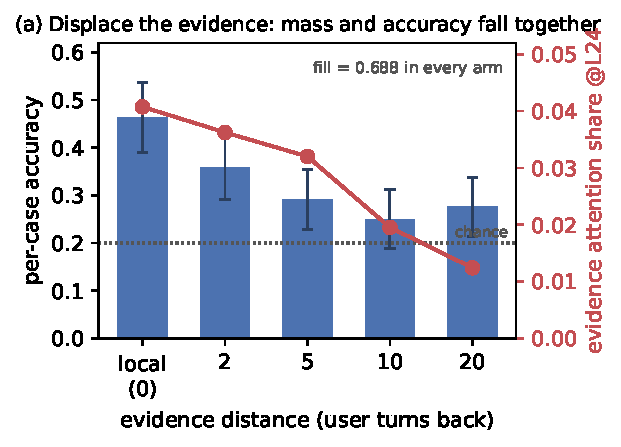
\includegraphics[width=\linewidth]{figures/distance_ladder.pdf}\end{subfigure}
  \hfill
  \begin{subfigure}{0.305\textwidth}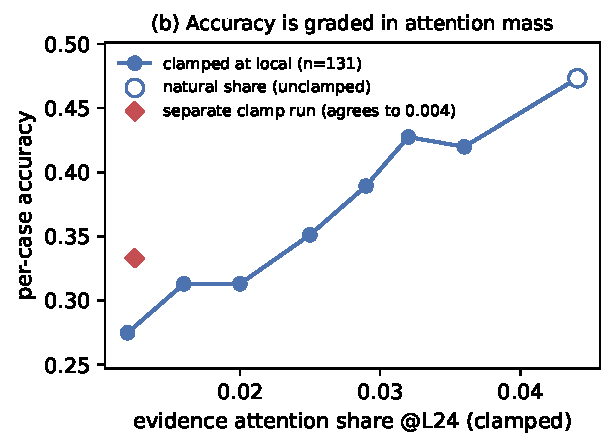
\includegraphics[width=\linewidth]{figures/mass_dose.pdf}\end{subfigure}
  \hfill
  \begin{subfigure}{0.305\textwidth}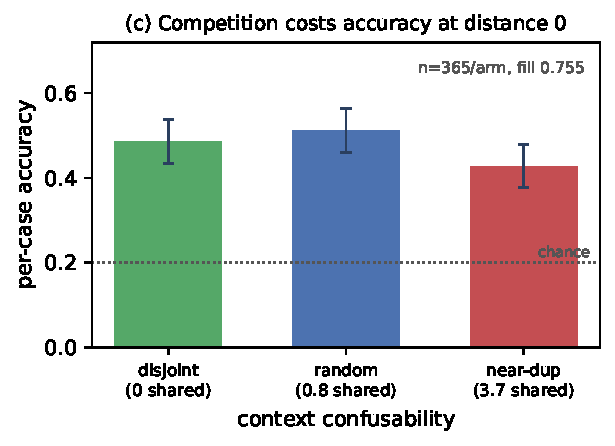
\includegraphics[width=\linewidth]{figures/competition.pdf}\end{subfigure}
  \caption{\textbf{Dilution costs accuracy. Accumulation does not.}
  (a) Moving the evidence $k$ user turns back, at identical fill and byte-identical questions,
  drains its attention mass and costs accuracy together.
  (b) Setting that mass directly, with the evidence left in place, reproduces the penalty and
  traces a smooth graded dose-response---no threshold. The diamond is the independently-run
  removal experiment's endpoint (agreement $0.004$ layer-24-indexed, $0.017$ all-layer).
  (c) At distance $0$ and fixed fill, near-duplicate accumulated context costs a further
  $0.085$. Bootstrap CIs resample cases throughout.}
  \label{fig:dilution}
\end{figure}

\subsection{Displacement acts through attention mass}
\label{sec:displacement}

We now vary only the position of the answer-bearing evidence. Each DDXPlus probe's vignette is
placed $k$ user turns before its question. Mean fill is $0.688$ in every arm, the question text is
byte-identical, and the overflow guard skipped $0$ of $192$ probes (example transcript in
Appendix~\ref{app:examples}). Every gap's CI excludes zero
(Table~\ref{tab:distance}, Fig.~\ref{fig:dilution}a). In a joint fit of accuracy on fill and
distance, distance carries the coefficient and fill carries none. Within the
\texttt{local} arm, the one that reproduces the accumulation design, accuracy is flat with
fill (Table~\ref{tab:fits}). The effect survives restriction to parsed responses and
is then fully monotone ($0.524\to0.413\to0.397\to0.343\to0.338$). The decline saturates by
$k{\approx}10$, where the $k{=}10$ and $k{=}20$ arms stop being distinguishable. The same
model, on the same items at the same fill, degrades only when the evidence is displaced. These
same items degrade as soon as dilution is reintroduced, which places \S\ref{sec:accumulation}'s
flat accuracy away from any ceiling.

Distance and attention drain move together by construction. Table~\ref{tab:distance} is
consistent with dilution but does not establish it, because a purely positional account
predicts the same table. Four interventions separate them.

\paragraph{Observational correlations.}
Evidence share falls $0.0408\to0.0124$ across the ladder ($r=-0.83$ with distance) while the
question's share stays flat, confirming only the evidence moved. One caution:
within an arm, higher evidence share predicts lower accuracy
($\beta=-11.2$ per unit share, and stronger controlling for vignette length). Attention there tracks
item difficulty (the model looks harder at confusing vignettes) and has the opposite sign
to the causal effect below.


\begin{table}[t]
  \centering\small
  \caption{\textbf{Removing the evidence's attention mass reproduces the displacement penalty;
  restoring it does not.} Paired contrasts in percentage points, all-layer shares, bootstrap
  95\% CIs over shared items ($n{=}192$; the sweep at $n{=}131$). Positive is accuracy lost.}
  \label{tab:mass}
  \setlength{\tabcolsep}{5pt}
  \begin{tabular}{lccc}
    \toprule
    contrast & $\Delta$ accuracy (pts) & 95\% CI & of penalty\\
    \midrule
    \texttt{local} $-$ clamped to \texttt{back\_20} share & $\mathbf{+15.1}$ & $[+9.9,+20.8]$ & $91\%$\\
    clamped $-$ \texttt{back\_20} & $+1.6$ & $[-5.2,+8.3]$ & ---\\
    natural $-$ sweep endpoint at displaced share & $+16.8$ & $[+10.2,+23.4]$ & ---\\
    restored to \texttt{local} share $-$ \texttt{back\_20} & $\mathbf{+4.7}$ & $[+1.0,+8.3]$ & $28\%$\\
    per-head restoration $-$ uniform clamp & $-2.1$ & $[-8.3,+4.2]$ & ---\\
    \bottomrule
  \end{tabular}
\end{table}

\paragraph{Mass removal.}
Keeping the evidence at \texttt{local} and clamping its share down to the same item's own
\texttt{back\_20} share reproduces the displacement penalty and lands the arm on
\texttt{back\_20} (Table~\ref{tab:mass}, paired $n{=}192$). \textbf{Mass removal alone
reproduces the displacement penalty, with nothing moved.}

\paragraph{Dose-response.}
Sweeping the evidence's share at fixed position over seven levels (layer-24-indexed, common
subset $n{=}131$ present
at every level) gives a graded decline from $0.473$ at the natural share ($0.0441$) to $0.275$ at
$0.012$ (Fig.~\ref{fig:dilution}b). Six of the seven levels differ significantly from the natural
share, including a cut of less than a fifth of the mass, and no step is a threshold: the largest
adjacent step is $0.053$ and the decline is smooth throughout. Its endpoint at the displaced
share matches the independently-run removal experiment in both denominations---to $0.4$
points layer-24-indexed and $1.7$ points on Table~\ref{tab:mass}'s all-layer scale.

\paragraph{Mass restoration.}
The converse is only partial: clamping the displaced evidence's share back up to its
\texttt{local} level recovers little of the penalty (Table~\ref{tab:mass}). The natural suspect is the instrument, since a uniform clamp cannot reconstruct which
heads should carry the restored mass. A pattern-matched test rules that out: one closed-form
bias per query head per layer, restoring each item to its donor's per-head pattern (mean
per-head share error $0.004$, bias SD $1.22$), gains nothing over the uniform clamp
(Table~\ref{tab:mass}).
Head identity is not what restoration is missing. One bias per head is still uniform over the
evidence's ${\sim}280$ tokens, and the remainder is either that within-span token pattern or a
positional channel outside attention altogether. The drain itself is positional in
tokens, not turns. A $64\%$ mass cut from token distance alone costs at most $9.4$
points, consistent with RoPE distance decay \citep{su2024rope,wu2025positionbias} rather than
conversation structure (Appendix~\ref{app:displacement-detail}). The ladder, the sufficiency
clamp ($107\%$ of the gap), and the graded dose-response all replicate on Qwen2.5-7B, there
with no unparsed replies (Appendix~\ref{app:qwen}).

\subsection{Competition acts through the competitors, not the evidence}
\label{sec:competition}

Burying a needle varies two things at once: the evidence becomes distant and it becomes
surrounded by plausible alternatives. We isolate the second by holding the evidence at the
current query and fill fixed, and varying only how confusable the accumulated context is.
Every arm accumulates eight prior DDXPlus cases, each answered in the transcript with its gold
letter, so format and in-context-learning affordance are constant. The arms differ only in how
much the accumulated cases' differentials overlap the probe's five options: \texttt{random}
(the natural stream, $0.80$ shared options on average), \texttt{disjoint} (zero), and
\texttt{near\_dup} (at least $3$, averaging $3.75$). No arm admits a context case with the
probe's own gold, so the manipulation is that in \texttt{near\_dup} the probe's gold routinely
appears as some context case's distractor (Appendix~\ref{app:tasks}). Paired
over $n{=}365$ probes, accuracy is \texttt{random} $0.512$, \texttt{disjoint} $0.485$,
\texttt{near\_dup} $\mathbf{0.427}$ (Fig.~\ref{fig:dilution}c).

Near-duplicate context costs $8.5$ points against the natural stream and $5.8$ against
disjoint context (intervals in Table~\ref{tab:intervals}). In a joint fit within this experiment, option
overlap carries the coefficient and fill carries none
(Table~\ref{tab:fits}), the same shape as the distance result on a different variable. Two
controls hold: the low-competition arms land on \S\ref{sec:displacement}'s \texttt{local}
accuracy of $0.464$ (both gaps n.s.), and \texttt{disjoint} is the longest arm while \texttt{near\_dup} is the shortest; length
works against the result. The effect survives restriction to parsed responses ($+8.2$ points, significant). It is not
monotone in confusability, with \texttt{random} sitting above \texttt{disjoint} (n.s.):
near-duplicate context is costly, and the cost does not track overlap.

\paragraph{The dissociation on mass.}
Repeating the sweep with attention capture (same probes, same seeds) separates the two
mechanisms on mass: displacement removes $4.55\%$ of the evidence's attention share and
competition removes $0.22\%$, while costing $18.8$ and $8.5$ accuracy points respectively---a
${\sim}20\times$ smaller mass change at half the accuracy cost, far too small to act through
the displacement dose-response. The two drain profiles are negatively correlated across layers
($r{=}-0.32$): displacement bites hardest at layers 0--3 and 16, competition at 17--18---opposite attention
signatures for the same accuracy contrast. Per-head structure, including the null result that no
head hides a large countervailing move, is in Appendix~\ref{app:heads}.

\begin{table}[t]
  \centering\small
  \caption{\textbf{What the closure recovers depends on what the closed tokens say, not on how
  much attention they hold.} Generation-time closures on the near-duplicate arm, paired
  $n{=}365$, every arm closing the same ${\approx}128$-token budget. Mass closed is a share of
  the final-position attention row; net accuracy is in percentage points against each arm's
  size-matched random control. Bold marks an interval excluding zero.}
  \label{tab:closures}
  \setlength{\tabcolsep}{5pt}
  \begin{tabular}{lccc}
    \toprule
    closed set & mass closed & net accuracy (pts) & 95\% CI\\
    \midrule
    verbatim option-name mentions & $0.77\%$ & $\mathbf{+6.0}$ & $[+0.8,+11.2]$\\
    verbatim, re-run alongside the arms below & $0.76\%$ & $\mathbf{+6.9}$ & $[+1.6,+12.1]$\\
    most-read content tokens & $8.7\%$ & $+0.3$ & $[-4.9,+5.5]$\\
    most-read tokens including template glue & $41.6\%$ & $\mathbf{-17.5}$ & $[-23.0,-12.1]$\\
    \bottomrule
  \end{tabular}
\end{table}

\paragraph{The competitor-closure test.}
An evidence-mass change this small rules out starvation as the carrier. It does not
touch the other attentional route,
in which the filler's (arm-constant) mass lands on instances of the probe's own answer
candidates and reading them is what misleads. We test this directly: closing every context
occurrence of the probe's option names at generation time recovers \textbf{56\%} of the
competition penalty (Table~\ref{tab:closures}), the residual gap to \texttt{random} no longer
excludes zero, and the rescue survives restriction to parsed responses. \textbf{Competition
is attention-mediated through the competitors, not the evidence}: less
than $1\%$ of the attention distribution carries the effect, and removing it removes most of
the cost. Both accuracy mechanisms are attentional, on different spans: displacement
removes mass from the evidence, competition directs mass onto the competitors, and the
evidence-mass measurement dissociates them because it is blind to the second by construction.
The ${\sim}40\%$ residual is not instrument slack of the high-attention kind: closing the
most-read content tokens of the context body, the same number of tokens as the
mentions and $8.7\%$ of the row's mass to their $0.76\%$, recovers
nothing (Table~\ref{tab:closures}). The closure works
through what the closed tokens say, not the mass they receive, and the residual
points at prefill-borne interference. The same measurement concentrates $42\%$ of
the entire final-position row in the ${\approx}128$ most-read tokens, dominated by the
chat template's turn delimiters. Closing that set is broadly destructive, but what it
disrupts is the demonstrated reply shape, not competition (\S\ref{sec:mode}).

\paragraph{The family divergence.}
Competition alone does not carry across families, and the divergence is itself informative. On the same $n{=}365$ panel Qwen2.5-7B shows no detected penalty
(\texttt{random} $-$ \texttt{near\_dup} $= +3.0$ points), and the scale-$0$
competitor closure that recovers $56\%$ of OLMo's penalty does nothing there ($+1.9$ points,
random-closure control $0.000$). The attention signatures separate with
disjoint intervals. Under near-duplicate context OLMo's evidence share is flat ($+0.0003$,
null) while Qwen's rises ($+0.0071$ in share, a disjoint interval), as if that model defends the
evidence under confusability rather than merely not paying for it
(Fig.~\ref{fig:qwen-replication}c,\,d). The families differ not by degree but in whether the competitor-reading channel is engaged at
all. We treat competition as architecture-indexed and rest its positive claims on OLMo
(Appendix~\ref{app:qwen}).

\subsection{Precedent: in-context learning against the system prompt}
\label{sec:precedent}

The costs so far are to accuracy. A third mechanism costs compliance: not whether the
model can still solve the task, but whether it answers in the instructed form
(\S\ref{sec:design}, $n{=}40$ probes per depth, one accumulation snapshotted at every depth, so
depth is the only mover).

Every stream here is also a stream of in-context examples. Each prior case is answered in the
transcript: the history demonstrates an answer shape while the system prompt
instructs one, two channels feeding one decision. When they agree, as in
\S\ref{sec:accumulation}'s compliant history, nothing surfaces. This section makes them
disagree, and the instruction gives way \citep[cf.][]{anil2024manyshot}.

\begin{table}[t]
  \centering\small
  \caption{\textbf{The instruction's attention decides the contest only while the transcript
  demonstrates nothing applicable.} $n{=}40$ per cell. Accumulation alone drives the system
  span's share $0.166\to0.021$ over eight turns, so row 2's clamped level is one the stream
  reaches by itself.}
  \label{tab:precedent}
  \setlength{\tabcolsep}{4pt}
  \begin{tabular}{llll}
    \toprule
    condition & compliance & accuracy & what it shows\\
    \midrule
    \multicolumn{4}{l}{\textit{no assistant turn in context}}\\
    system span at its natural $0.165$ & $0.99$ & $0.525$ & the instruction governs a silent transcript\\
    clamped to share $0.050$ & $0.03$ & $0.467$ & its attention is causally necessary\\
    \midrule
    \multicolumn{4}{l}{\textit{accumulated filler, at matched fill ${\approx}0.5$}}\\
    \texttt{code}, no applicable shape & $1.00$ & --- & erosion tracks how far the demonstrated\\
    \texttt{gsm8k}, loosely applicable & $0.60$ & --- & \quad shape transfers to the probe, not the\\
    \texttt{mmlu}, a drop-in replacement & $0.00$ & --- & \quad instruction's attention\\
    \midrule
    \multicolumn{4}{l}{\textit{at depth $42$, reversing it}}\\
    natural & $0.000$ & $0.650$ & the eroded floor\\
    clamp the system span back up & $1.000$ & $0.425$ & re-weighting reverses it, zero-sum in accuracy\\
    restate the instruction & $1.000$ & $0.450$ & re-presenting reverses it, without surgery\\
    both levers & $1.000$ & $0.275$ & the two costs add\\
    \bottomrule
  \end{tabular}
\end{table}

\paragraph{Attention decides the contest only when nothing is demonstrated.}
In a context with no assistant turn, clamping the system span collapses compliance with
accuracy unchanged and parsing at $0.967$ (a suffix canary flips on $120$ of $120$ items). The
clamped level is one accumulation passes on its own between two and four turns ($-2.6$ nats),
well clear of the near-ablation regime excluded in \S\ref{sec:displacement}. This confirms
\citet{dongre2026attentioncloses}'s ablation finding that system-prompt attention is causally
necessary, and sharpens it: the collapse needs no masking, only a graded clamp to a share
accumulation reaches by itself. Put one example in the transcript and the clamp stops
mattering. A single compliant example pins compliance at ceiling at every clamp level and a
single bare-letter example pins it at floor even unclamped, replies byte-copying the previous
assistant turn's format at zero length variance across $720$ generations per arm
(Appendix~\ref{app:precedent-detail}). The instruction governs behaviour only when the
transcript is silent.

\paragraph{What decides it instead is applicability.}
Three filler streams vary how far the demonstrated shape transfers to a $5$-option probe:
\texttt{code} (request$\to$Python function), \texttt{gsm8k} (worked prose), \texttt{mmlu}
(MCQ$\to$bare letter). Compliance follows that ordering rather than attention. \texttt{mmlu}
collapses $0.875\to0.000$ within three filler turns (fill $0.147$) and never recovers through
fill $0.87$, while \texttt{code} still holds $0.900$ at fill $0.778$
(Fig.~\ref{fig:erosion}a). Accuracy is unharmed throughout: the model still solves the case
and answers in the demonstrated style. The system prompt's attention does not carry the
difference, since its raw share falls on the same arithmetic curve in every arm, its per-token
enrichment is flat-to-rising in all three (Fig.~\ref{fig:erosion}b), and \texttt{code} holds
full compliance at half the raw share at which \texttt{mmlu} has already collapsed. The same model at the same near-zero share survives or collapses depending on what the filler
demonstrates, an axis \citet{dongre2026attentioncloses}'s fixed filler cannot see. Natural
dilution does not cause the erosion, being identical in the arm that never erodes.

Either lever reverses it in full (Fig.~\ref{fig:erosion}c), which makes attention mass a causal
weight in the contest: clamp the instruction down and it loses unopposed, clamp it up and it
wins against $42$ counter-exemplars, leave it natural and the demonstrated template beats it.
Re-presenting beats re-weighting, since mass forced onto a $48$-token span is taken from
everything else by \S\ref{sec:displacement}'s zero-sum arithmetic while a restatement costs the
model nothing. The applicability ordering, the reading signature, and restatement's advantage
all replicate on Qwen2.5-7B, where the erosion is staged rather than total
(Appendix~\ref{app:qwen}).

\subsection{The mode: readable, installable, not erasable}
\label{sec:mode}

We call the behavioral state \S\ref{sec:precedent} leaves behind the mode: the disposition to
answer in the demonstrated shape rather than the instructed one. Table~\ref{tab:mode} is the
search for it. Nine operations divide cleanly. Every operation on attention to the
demonstrated answers leaves compliance at the eroded floor, in any window. Every operation on
the residual stream moves it, reads it, or fails only at erasure.

\begin{table}[t]
  \centering\small
  \caption{\textbf{The mode is readable and installable, but not reachable through attention
  to the demonstrated answers.} Compliance at depth $42$ ($n{=}40$ per arm) unless noted;
  closures are scale-$0$ at generation time against size-matched random controls.
  Enrichment is \texttt{mmlu}/\texttt{gsm8k}/\texttt{code}, the erosion ordering of \S\ref{sec:precedent}.}
  \label{tab:mode}
  \setlength{\tabcolsep}{4pt}
  \begin{tabular}{lll}
    \toprule
    operation & outcome & what it shows\\
    \midrule
    \multicolumn{3}{l}{\textit{on attention to the demonstrated answers}}\\
    read out, per-token enrichment & $+1.28$/$+0.34$/neg. & they are read in the erosion order\\
    close at decode & compliance $0.000$ & reading does not sustain the mode\\
    close at prefill, decode, or both & $0.000$ in every window & reading does not install it\\
    the same closure, on accuracy & $-17.5$ pts prefill, $0.0$ decode & the reading is worth accuracy, not format\\
    \midrule
    \multicolumn{3}{l}{\textit{on the residual stream}}\\
    probe the instruction's presence & transfer AUC $1.000$ & represented at every depth, overruled\\
    probe the upcoming reply & LOO AUC $0.875$ & the outcome is fixed before the first token\\
    steer, mean-difference vector & $0.000$ vs.\ $0.425$ control & the mode is installable by direction\\
    erase, four projections & every one null & it is not erasable as a direction\\
    patch the template glue positions & $62\%$ of the full patch & the carrier is positional\\
    \bottomrule
  \end{tabular}
\end{table}

That split is the sharpest dissociation in the paper, because the operation on the left of it
is the one that worked in \S\ref{sec:competition}: the same scale-$0$ closure that recovers
$56\%$ of the competition penalty restores nothing here, in any window
(Fig.~\ref{fig:closure-dissociation}). Competition is generation-time reading. The precedent
mode is in place by prefill, a template already installed, task-vector style
\citep{hendel2023taskvectors}, through some channel other than attention to the answer spans.
The probe rows say the instruction is read, represented, and overruled, and that the outcome
is decidable from the residual stream before the first token is emitted. The erase nulls are
not redundancy: two fitted projections drive the layer's linear code to chance while the
behavior is untouched (Appendix~\ref{app:precedent-detail}), so the code is low-rank and the
behavioral decision does not consume the linearly decodable component. We can decode the mode
and we can install it. Neither shows what carries it.

\paragraph{The carrier, localized in tokens.}
What direction-level search could not find, position-level search does---on the second family,
where a counterfactual patching instrument exists (Appendix~\ref{app:qwen}): transplanting
per-position hidden states between two transcripts identical except for their format
instruction, and reading out the instructed formats' log-probability contrast
(Table~\ref{tab:patch}). The chat template's turn delimiters (the
\texttt{im\_end}/\texttt{im\_start} glue, holding no instruction text and no demonstrated
answer) carry $62\%$ of the full-context patch, every content subset carries at most $12\%$,
and the crossed cell of glue positions at layers $7$--$13$ still carries $42\%$. The format
state rides the transcript's skeleton, tokens the chat template already supplies, consistent
with delimiter and low-information tokens serving as computation slots
(Appendix~\ref{app:related}), and it is where the OLMo attention row concentrates
(\S\ref{sec:competition}, Fig.~\ref{fig:token-heatmap}). Unlike the mass absorbed by attention
sinks \citep{xiao2023streamingllm,gu2024attentionsink}, which is content-independent
normalization slack, the glue state is content-bearing and transportable: moving it moves the
behavior. The channel is cross-family. On OLMo, whose full-transcript effect is an order of
magnitude smaller and not inverted, the glue-only patch carries all of it ($+0.092$, $n{=}85$
after skips, vs.\ the full patch's $+0.056$, $n{=}34$, with the unrelated-fact control at
$-0.011$ in both).

\subsection{Why context rot gets reported: the signatures}
\label{sec:signatures}

\looseness=-1
A generic depth effect would survive on heterogeneous dialogue, and the entropy collapse
behind the context-rot reports does not. On 150 organic WildChat conversations
\citep{zhao2024wildchat}, within-conversation entropy is flat with depth (median late/early
ratio $0.99$). Partitioning a second, $400$-conversation run by its
own inter-turn homogeneity separates the driver: homogeneous tertiles collapse ($0.897$
late/early) while heterogeneous ones are flat ($1.001$, $n{=}134$ each). Because homogeneous
conversations are longer, length works against the effect. Across OLMo-2's
\citep{olmo2024} post-training chain the collapse is mostly a downward level shift in
baseline entropy installed by alignment, not a steeper slope
(Appendix~\ref{app:signatures-detail}).

\looseness=-1
The residual hazard in the localized case is calibration, not competence. On the DDXPlus
streams logging per-token confidence ($n{=}154$ pooled cases, two models, both question orders),
answer confidence rises $0.85\to0.95$ with fill ($r=+0.72$) at flat accuracy, and equally on
wrong answers ($0.86\to0.95$, $r=+0.69$): confidence in wrong answers rises ${\sim}10$
points over a session (Fig.~\ref{fig:signatures}c), most consequential where a homogeneous
high-stakes stream makes the model surest.

\section{Conclusion}

\looseness=-1
With accumulation, displacement, competition and precedent separated inside one harness, each
mechanism leaves a distinct signature:
\begin{itemize}[leftmargin=1.35em,itemsep=1pt,topsep=2pt]
\item \textbf{Accumulation} produces a monotone reallocation of attention and a collapse of
  predictive entropy, but no detected loss of accuracy and no loss of instruction
  adherence---the with-length decline that motivates the rot framing
  \citep{liu2023lost,hong2025contextrot,laban2025lost} does not surface in these streams.
\item \textbf{Displacement}, the retrieval case, produces a large accuracy cost that is
  reproduced in full by removing the evidence's attention mass, graded in that mass, and
  positional in tokens. This is the one mechanism that is attention dilution proper.
\item \textbf{Competition} produces a further cost while the evidence's attention barely
  moves: interference that raw context length does not index
  \citep[cf.][]{wang2025unabletoforget}, carried instead by attention to the competing
  instances themselves, under $1\%$ of the distribution.
\item \textbf{Precedent} erodes not accuracy but compliance, in a contest the
  instruction loses with its attention intact: the benign, self-generated counterpart
  of demonstrations overriding priors and instructions
  \citep{wei2023icldifferently,anil2024manyshot,camassa2026instructioninduction}.
\end{itemize}
The literature's central claim is correct but misattributed and undercounted. In
these streams, context rot is not a decay with length: it is three mechanisms with different
signatures, of which length is merely the usual way of causing all three at once. A needle
buried far away among plausible alternatives moves the displacement and competition levers
at once, and length-indexed benchmarks cannot separate them
\citep{hsieh2024ruler}; attention-share accounts of multi-turn decline
\citep{dongre2026attentioncloses} describe only the mechanism that is dilution proper. The
precedent state itself, unreachable as a direction, is reachable as a place: the transcript's
skeleton electing itself as native instruction storage
\citep{darcet2023registers,sun2024massiveactivations,mu2023gist}.
Displacement, its mass sufficiency, the accumulation null, and the precedent contest replicate
on a second model family. Competition is the mechanism that does not: it is
architecture-indexed, its attention signature inverting on Qwen (Appendix~\ref{app:qwen}).

\section{Limitations}
\label{sec:limitations}

\looseness=-1
Per-condition $n$ is bounded by the window, and every interval depends on
\S\ref{sec:design}'s paired analysis. The accumulation null resolves declines above $2.9$
points (coherent) and $5.5$ (random); its random-subject control leaves format and protocol
learning available in both streams. For displacement, removal establishes sufficiency in full
while restoration returns $0.28$ of the penalty. Head-uniformity is excluded as the clamp's
limitation, but it still spreads restored mass uniformly over the span's tokens, leaving a
within-span token pattern and a non-attention positional channel unseparated. The competition result is one significant step rather than a gradient: mild overlap
is indistinguishable from none, and the near-duplicate arm changes the selection regime.
Its closure rescue leaves ${\sim}40\%$ of the gap unexplained, and the hot-set control,
ranked on the all-layer mean row, leaves a low-mass paraphrase channel open. The instruction-canary null is a floor effect, the WildChat partition is observational with no
uncertainty on the tertile contrast, competition rests on one family, and the low-share
compliance dissociation is OLMo-specific (Appendix~\ref{app:qwen}).

\looseness=-1
The precedent results use one instruction family at $n{=}40$ per cell, and the filler streams
co-vary in genre, structure, and reply length, leaving the applicability ordering resting on
the stream contrast with the one-example and reversal experiments. Window-split closure rules
out exemplar-answer attention for that span family only. The carrier localization is confounded with
positional periodicity, its patch readout is teacher-forced, and the mechanisms are ranked at
\S\ref{sec:design}'s $4$k window rather than at $128$k.

% The style prints this only under [final] or [preprint] and hides it in every submission mode.
\begin{ack}
This work was carried out in the Supervised Program for Alignment Research (SPAR). The author
thanks Justin Shenk for mentorship and feedback throughout the project, and the SPAR
organizers for making it possible.
\end{ack}

\small
\begin{thebibliography}{9}
\bibitem[Agarwal et al.(2024)]{agarwal2024manyshot} R.~Agarwal et al. Many-shot in-context learning. \emph{NeurIPS}, 2024.
\bibitem[Alain and Bengio(2016)]{alain2016probes} G.~Alain and Y.~Bengio. Understanding intermediate layers using linear classifier probes. \emph{arXiv:1610.01644}, 2016.
\bibitem[Anil et al.(2024)]{anil2024manyshot} C.~Anil et al. Many-shot jailbreaking. \emph{NeurIPS}, 2024.
\bibitem[Belinkov(2022)]{belinkov2022probing} Y.~Belinkov. Probing classifiers: promises, shortcomings, and advances. \emph{Computational Linguistics}, 48(1), 2022.
\bibitem[Camassa and Shiller(2026)]{camassa2026instructioninduction} A.~Camassa and B.~Shiller. Do as I say, not as I do: instruction-induction conflict in LLMs. \emph{arXiv:2605.20382}, 2026.
\bibitem[Cuconasu et al.(2024)]{cuconasu2024noise} F.~Cuconasu et al. The power of noise: redefining retrieval for RAG systems. \emph{SIGIR}, 2024.
\bibitem[Darcet et al.(2024)]{darcet2023registers} T.~Darcet, M.~Oquab, J.~Mairal, and P.~Bojanowski. Vision transformers need registers. \emph{ICLR}, 2024.
\bibitem[Davidson et al.(2025)]{davidson2025taskrepresentation} G.~Davidson, T.~Gureckis, B.~Lake, and A.~Williams. Do different prompting methods yield a common task representation in language models? \emph{NeurIPS}, 2025.
\bibitem[Dongre et al.(2026)]{dongre2026attentioncloses} V.~Dongre et al. When attention closes: how LLMs lose the thread in multi-turn interaction. \emph{arXiv:2605.12922}, 2026.
\bibitem[Grattafiori et al.(2024)]{llama3herd} A.~Grattafiori et al. The Llama 3 herd of models. \emph{arXiv:2407.21783}, 2024.
\bibitem[Gu et al.(2025)]{gu2024attentionsink} X.~Gu et al. When attention sink emerges in language models: an empirical view. \emph{ICLR}, 2025.
\bibitem[Hendel et al.(2023)]{hendel2023taskvectors} R.~Hendel, M.~Geva, and A.~Globerson. In-context learning creates task vectors. \emph{Findings of EMNLP}, 2023.
\bibitem[Hendrycks et al.(2021)]{hendrycks2021mmlu} D.~Hendrycks et al. Measuring massive multitask language understanding. \emph{ICLR}, 2021.
\bibitem[Hong et al.(2025)]{hong2025contextrot} K.~Hong, A.~Troynikov, and J.~Huber. Context rot: how increasing input tokens impacts LLM performance. Chroma technical report, 2025.
\bibitem[Hsieh et al.(2024a)]{hsieh2024foundinmiddle} C.-Y.~Hsieh et al. Found in the middle: calibrating positional attention bias improves long context utilization. \emph{Findings of ACL}, 2024.
\bibitem[Hsieh et al.(2024b)]{hsieh2024ruler} C.-P.~Hsieh et al. RULER: what's the real context size of your long-context language models? \emph{COLM}, 2024.
\bibitem[Laban et al.(2025)]{laban2025lost} P.~Laban, H.~Hayashi, Y.~Zhou, and J.~Neville. LLMs get lost in multi-turn conversation. \emph{arXiv:2505.06120}, 2025.
\bibitem[Levy et al.(2024)]{levy2024same} M.~Levy, A.~Jacoby, and Y.~Goldberg. Same task, more tokens: the impact of input length on the reasoning performance of large language models. \emph{ACL}, 2024.
\bibitem[Liu et al.(2023)]{liu2023lost} N.~F. Liu et al. Lost in the middle: how language models use long contexts. \emph{TACL}, 2023.
\bibitem[Lieberum et al.(2024)]{lieberum2024gemmascope} T.~Lieberum et al. Gemma Scope: open sparse autoencoders everywhere all at once on Gemma 2. 2024.
\bibitem[Meng et al.(2022)]{meng2022rome} K.~Meng, D.~Bau, A.~Andonian, and Y.~Belinkov. Locating and editing factual associations in GPT. \emph{NeurIPS}, 2022.
\bibitem[Mu et al.(2023)]{mu2023gist} J.~Mu, X.~L. Li, and N.~Goodman. Learning to compress prompts with gist tokens. \emph{NeurIPS}, 2023.
\bibitem[Mu et al.(2025)]{mu2025systemprompt} N.~Mu et al. A closer look at system prompt robustness. \emph{arXiv:2502.12197}, 2025.
\bibitem[Olsson et al.(2022)]{olsson2022induction} C.~Olsson et al. In-context learning and induction heads. \emph{arXiv:2209.11895}, 2022.
\bibitem[Shi et al.(2023)]{shi2023distracted} F.~Shi et al. Large language models can be easily distracted by irrelevant context. \emph{ICML}, 2023.
\bibitem[Su et al.(2024)]{su2024rope} J.~Su et al. RoFormer: enhanced transformer with rotary position embedding. \emph{Neurocomputing}, 568, 2024.
\bibitem[Sun et al.(2024)]{sun2024massiveactivations} M.~Sun, X.~Chen, J.~Z. Kolter, and Z.~Liu. Massive activations in large language models. \emph{arXiv:2402.17762}, 2024.
\bibitem[Tchango et al.(2022)]{tchango2022ddxplus} A.~Fansi Tchango et al. DDXPlus: a new dataset for automatic medical diagnosis. \emph{NeurIPS Datasets and Benchmarks}, 2022.
\bibitem[Team OLMo(2024)]{olmo2024} Team OLMo et al. 2 OLMo 2 Furious. \emph{arXiv:2501.00656}, 2024.
\bibitem[Todd et al.(2024)]{todd2024functionvectors} E.~Todd et al. Function vectors in large language models. \emph{ICLR}, 2024.
\bibitem[Vig et al.(2020)]{vig2020mediation} J.~Vig et al. Investigating gender bias in language models using causal mediation analysis. \emph{NeurIPS}, 2020.
\bibitem[Wang and Sun(2025)]{wang2025unabletoforget} C.~Wang and Y.~Sun. Unable to forget: proactive interference reveals working memory limits in LLMs beyond context length. \emph{ICML Workshop on Long-Context Foundation Models}, 2025.
\bibitem[Wang et al.(2023)]{wang2023ioi} K.~Wang, A.~Variengien, A.~Conmy, B.~Shlegeris, and J.~Steinhardt. Interpretability in the wild: a circuit for indirect object identification in GPT-2 small. \emph{ICLR}, 2023.
\bibitem[Wei et al.(2023)]{wei2023icldifferently} J.~Wei et al. Larger language models do in-context learning differently. \emph{arXiv:2303.03846}, 2023.
\bibitem[Wu et al.(2025)]{wu2025positionbias} X.~Wu, Y.~Wang, S.~Jegelka, and A.~Jadbabaie. On the emergence of position bias in transformers. \emph{ICML}, 2025.
\bibitem[Xiao et al.(2024)]{xiao2023streamingllm} G.~Xiao et al. Efficient streaming language models with attention sinks. \emph{ICLR}, 2024.
\bibitem[Yang et al.(2024)]{qwen2025} A.~Yang et al. Qwen2.5 technical report. \emph{arXiv:2412.15115}, 2024.
\bibitem[Zhang and Nanda(2024)]{zhang2024patching} F.~Zhang and N.~Nanda. Towards best practices of activation patching in language models: metrics and methods. \emph{ICLR}, 2024.
\bibitem[Zhang et al.(2024)]{zhang2023pasta} Q.~Zhang et al. Tell your model where to attend: post-hoc attention steering for LLMs. \emph{ICLR}, 2024.
\bibitem[Zhao et al.(2024)]{zhao2024wildchat} W.~Zhao et al. WildChat: 1M ChatGPT interaction logs in the wild. \emph{ICLR}, 2024.
\end{thebibliography}

\appendix
\normalsize
\raggedbottom

\paragraph{Code and artifacts.}
The harness, the span-attention clamp, every driver behind the experiments, and the committed
run artifacts (per-turn CSVs and summaries) that each number in this paper traces to are at
\url{\repourl}.

\section{Background and related work}
\label{app:related}

\paragraph{Length as the suspected cause.}
Most evidence for context rot comes from setups where the answer-bearing information sits inside
a single long input. \citet{liu2023lost} showed that accuracy depends strongly on where in
the context the relevant passage sits, dipping when it falls in the middle. \citet{levy2024same}
held a reasoning task fixed and padded the input with task-irrelevant text, finding degradation
well before the models' advertised context limits. \citet{hong2025contextrot} ran a broad sweep
over 18 models and found that reliability falls with input length even on tasks as simple as
retrieval and replication, and that the fall is not uniform: it depends on how similar the needle
is to the question, and on whether distractors are present. \citet{hsieh2024ruler} show the
benchmark-level version: near-perfect needle scores coexist with sharp degradation on harder
long-context tasks, and claimed context sizes overstate usable ones. \citet{laban2025lost} report a large
multi-turn degradation, but locate its cause in the model committing early to a wrong reading and
failing to recover---not in length as such.

\paragraph{Confusable context as a separate suspect.}
A second literature manipulates the content of the surrounding context rather than its
length. \citet{shi2023distracted} insert an irrelevant sentence into grade-school math problems
and observe a sharp accuracy drop. In retrieval-augmented generation, \citet{cuconasu2024noise}
find that documents retrieved as relevant but not containing the answer act as distractors and
degrade accuracy. \citet{wang2025unabletoforget} show accuracy declining log-linearly as
interfering similar updates accumulate, independent of raw context length---the nearest neighbor
to our competition result, with no attention instrumentation. Our contribution is to locate the
cost: it runs at held-constant evidence attention mass and is carried by attention to the
competing instances themselves (\S\ref{sec:competition}).

\paragraph{Instructions versus demonstrations.}
Demonstrations can override a model's trained priors \citep{wei2023icldifferently} and, at
scale, its safety training \citep{anil2024manyshot}. The same lever is framed as pure benefit in
many-shot prompting \citep{agarwal2024manyshot}. Hardcoded assistant turns exhibiting a
competing pattern flip instruction-following into pattern-following
\citep{camassa2026instructioninduction}, system-prompt adherence fails under conflicting or
adversarial user turns \citep{mu2025systemprompt}, and instruction-derived and
demonstration-derived task representations are measurably distinct
\citep{davidson2025taskrepresentation}. Our eroding pressure differs from all of these: it is
benign, self-generated, and contains no conflicting directive anywhere. It is precedent, not
conflict or attack, and we identify the contest's causal weight and both of its reversals.

\paragraph{Attention as measurement and lever.}
Closest to our mechanistic question, \citet{dongre2026attentioncloses} track attention from
responses to the system prompt declining over $50$ filler turns across four model families, show
that hard-masking the instruction out of the window collapses compliance, and decode goal
information from the residual stream at high AUC after attention has ``closed''. Our design differs in three ways. Their goal-accessibility metric aggregates raw share, which falls by
arithmetic as context grows (\S\ref{sec:share}). Our token-normalized enrichment removes that
decline entirely, and the corrected quantity is flat in eroding and non-eroding arms alike.
Their causal arm is total ablation (attention necessary, which our system-span clamp
confirms), while our clamp is graded and bidirectional, and the restoration direction
(compliance recovered against $42$ counter-exemplars) is an arm ablation cannot supply. Their filler is always inapplicable. Our applicability ladder shows the same model at the same
near-zero share surviving or collapsing depending on what the filler demonstrates, a content
dependence invisible to fixed-filler designs. On the steering side, \citet{zhang2023pasta} boost
attention on profiled head subsets to improve compliance and \citet{hsieh2024foundinmiddle}
recalibrate a static positional attention bias globally. Our clamp is the measurement-grade
counterpart (bit-identical no-op, solvable dose, span-targeted in accumulating multi-turn
context), used to establish when attention mass is and is not the mediating variable.
Position-driven attention structure is the content-independent backdrop to all of this: sink
tokens absorb mass regardless of content \citep{xiao2023streamingllm,gu2024attentionsink}, and
the causal mask plus RoPE produce distance decay by construction \citep{wu2025positionbias}.
Our clamps and token-normalized shares target content spans against that backdrop.

\paragraph{Compact task representations.}
In-context demonstrations compress into residual task vectors \citep{hendel2023taskvectors}
transported by identifiable heads \citep{todd2024functionvectors}. These are the
no-attention-signature channel our precedent mechanism
appears to use (\S\ref{sec:mode}), and our erase-null results bound what such compact readable
structure can be assumed to do causally. The byte-exact format copying our pinned arms show
(Appendix~\ref{app:precedent-detail}) is the behavior induction heads implement at circuit
level \citep{olsson2022induction}. We implicate that circuit behaviorally and at span level,
without head-level verification.

\section{Instrument validation}
\label{app:instruments}

\paragraph{Attention capture.}
Shares are read from a reconstruction of each layer's attention at the final position, which
avoids materializing $N\times N$ attention matrices. With $\tilde q$ and $\tilde K$ the
final-position query and the keys after QK-norm (where the architecture applies it) and RoPE,
and $m$ the additive attention mask, the reconstructed row is
\[
  a \;=\; \mathrm{softmax}\!\left(\frac{\tilde q\,\tilde K^{\top}}{\sqrt{d}} + m\right).
\] The reconstruction matches the
framework's own \texttt{output\_attentions} rows to max $|\Delta| = 1.1\times10^{-6}$ on OLMo-2
and $3.1\times10^{-5}$ on a GQA architecture (Qwen-2), both in fp32. Including $m$ makes the capture valid under a mask-based intervention: a capture that
ignores the mask still matches on plain forwards, where a causal mask's last query row is all
zeros, while silently reporting unclamped attention during a clamp.

\paragraph{Clamp.}
At scale $1.0$ the clamp is bit-identical to the unhooked model (max $|\Delta|$ logits $=0.0$),
because it adds $b{=}0$ to the existing mask rather than reimplementing attention
(\S\ref{sec:clamp}). The bias is
uniform across heads, and a span's aggregate share is hit by bisection on $b$. All solved levels
in this paper land within ${\sim}10^{-4}$ of target. Setting a span's scale to $0$ fills its key
columns with the mask minimum---closure, the same operation as a causal mask. Interpretation is
restricted to biases well clear of near-ablation: levels requiring $-4.7$ to $-6.1$ nats produce
degenerate behavior (the model answers ``A'' on $103$--$110$ of $110$ items) and are excluded.

\section{Task and filler specifications}
\label{app:tasks}

\paragraph{Probe construction.}
DDXPlus probes are $5$-option differentials with the vignette as evidence. Options are shuffled
per probe: DDXPlus lists the differential in rank order, so unshuffled gold is the letter ``A''
in $71.4\%$ of probes, and arms that differ in letter bias then differ in accuracy for free.
Items with fewer than $5$ options are excluded ($26.7\%$ of raw cases, some answerable from
a single option without the vignette). Generation budgets are per-protocol: the accuracy arms
(\S\ref{sec:displacement}--\S\ref{sec:competition}) generate $32$ new tokens. The compliance
arms (\S\ref{sec:precedent}) generate $128$ for the probe reply (fillers up to $200$), because
shorter caps truncate the reply component that formats put last, biasing exactly the metric
under study. The probe and steering runs (Appendix~\ref{app:precedent-detail}) generate $256$.

\paragraph{Format instruction and grader.}
The clinical template requires \texttt{ANSWER:} with a letter and \texttt{SUPPORTING:} with at
least two findings quoted from the vignette. Compliance requires the template. Accuracy is
scored separately and more permissively (a letter offered in prose, or alone on the reply's
first line, is scoreable for accuracy while remaining non-compliant). The grader was validated
against real generations from every condition. Graders written against imagined output formats
systematically mis-score exactly the conditions where the treatment changes the output format.

\paragraph{Filler streams.}
Filler replies are the model's own (up to $200$ tokens, \texttt{mmlu} answers truncated to the
letter), so each arm demonstrates the shape the model itself produces for that stream rather
than a shape we wrote. Table~\ref{tab:filler} gives the three. Applicability is the design
variable: it is the only thing that separates the arms, and it is what \S\ref{sec:precedent}
shows the erosion follows.

\begin{table}[H]
  \centering\small
  \caption{\textbf{The three filler streams, ordered by how far their demonstrated answer
  shape transfers to a $5$-option probe.} Fill per turn differs by ${\approx}3\times$, so the
  arms are compared at matched fill rather than matched depth.}
  \label{tab:filler}
  \setlength{\tabcolsep}{5pt}
  \begin{tabular}{lllll}
    \toprule
    stream & source & demonstrated reply & applicable to the probe? & fill/turn\\
    \midrule
    \texttt{code} & 30 synthetic request$\to$function & a Python function & no shape in common & ${\sim}0.056$\\
    \texttt{gsm8k} & grade-school math & worked prose & loosely, via prose & ${\sim}0.030$\\
    \texttt{mmlu} & 4-option MCQ, non-medical & a bare letter & a drop-in replacement & ${\sim}0.018$\\
    \bottomrule
  \end{tabular}
\end{table}

\paragraph{Canaries.}
The system-clamp arms use a three-part canary instruction (reply prefix marker, suffix tag,
and a forbidden phrase). The adherence arm uses the prefix and suffix pair. The
forbidden-phrase canary is satisfied trivially by short
replies, so two canaries are informative.

\paragraph{Run configuration.}
The settings that hold across the whole program, gathered here because they are otherwise
stated where they are first used. The primary model is
\texttt{allenai/OLMo-2-1124-7B-Instruct} and the replication model
\texttt{Qwen/Qwen2.5-7B-Instruct}, both at seed 42 with greedy decoding. Every mechanism
experiment runs in a $4$k window on both families; the two departures are not mechanism
results, the adherence arm of \S\ref{sec:accumulation} at $32$k and the WildChat measurements
at $16$k and $32$k. An attention share is the post-softmax mass at the final position, meaned
over heads and pooled over all $32$ layers, with layer 24 read as a reference in the ladder
diagnostics, and the clamp is uniform across heads and applied at every layer unless stated
otherwise. All contrasts are paired over shared items, all intervals are case-resampled
bootstraps at $10{,}000$ draws ($4{,}000$ for fit coefficients), and the overflow guard skips
any item that would not fit whole rather than truncating it. Probe construction and the
per-protocol generation budgets are above; the drop counts are in
Appendix~\ref{app:stats}.


\section{Example transcripts and generations}
\label{app:examples}

Both examples are the first probe of their committed runs, reconstructed byte-exactly from the
run's seed and validated against the stored artifacts (token counts, pathology, gold). The
generations are quoted verbatim from each run's stored \texttt{turns.csv}, truncated where the
$32$-token generation cap truncated them. Transcripts are abridged, and $[\dots]$ marks elided
text.

\paragraph{Displacement (\S\ref{sec:displacement}).}
Session 0's first depth-21 probe: gold D (acute pulmonary edema), fill $0.50$ in every arm.
The transcript accumulates $21$ answered MMLU filler exchanges. The vignette and the question
are byte-identical across arms and only the vignette's position differs---in \texttt{local} it
is the user turn directly before the question, in \texttt{back\_10} the same turn sits ten
filler exchanges earlier.

\begin{quote}\small
\texttt{[user]} You are answering a mixed stream of questions. Some are multiple-choice
knowledge questions; some describe a patient. Answer each one as it arrives.\par\smallskip
\texttt{[assistant]} Understood.\par\smallskip
\texttt{[user]} Which of the following ions CANNOT be used as a dopant in germanium to make an
n-type semiconductor? A) As B) P C) Sb D) B. Reply with only the letter\dots\par\smallskip
\texttt{[assistant]} D\par\smallskip
$[\dots\text{19 more filler exchanges}\dots]$\par\smallskip
\texttt{[user]} Patient: 76-year-old Female. Chief complaint: Are your symptoms worse when
lying down and alleviated while sitting up. Symptoms: pain (tedious, sensitive, heavy) in the
lower and posterior chest, intensity 9, radiating to biceps, chin, jaw, shoulders; shortness of
breath; bouts of choking that wake you up at night; swelling in ankles, calves, tibia
$[\dots]$ History: fluid in the lungs; dialysis; high blood pressure; heart attack or angina;
heart failure $[\dots]$\par\smallskip
\texttt{[assistant]} Noted.\par\smallskip
\texttt{[user]} For the patient described earlier, most likely diagnosis: A) Pulmonary
embolism B) Possible NSTEMI / STEMI C) Anaphylaxis D) Acute pulmonary edema E) Pericarditis.
Answer:
\end{quote}

\noindent In \texttt{back\_10} the vignette turn and its \texttt{Noted.} sit above ten of the
filler exchanges instead of none. The generations for this item:

\begin{quote}\small
\texttt{local:} ``D'' \hfill (parsed, correct)\par\smallskip
\texttt{back\_10:} ``Given the symptoms described for the patient, such as sudden onset of
severe chest pain that is worse when lying down and alleviated by sitting up, shortness of''
\hfill (unparsed, wrong)
\end{quote}

\noindent The displaced reply paraphrases the vignette accurately, so the model is not blind to
the evidence, but it never commits to a letter. \texttt{back\_2}, \texttt{back\_5} and
\texttt{back\_20} fail the same way on this item. This is the unparsed failure mode whose rate
rises with fill. The ladder survives restriction to parsed responses (\S\ref{sec:displacement}),
where the failures are wrong letters instead.

\paragraph{Competition (\S\ref{sec:competition}).}
Probe 0: gold E (viral pharyngitis). Every arm holds the vignette at the current query
(distance $0$) and accumulates eight answered DDXPlus cases. Only option overlap differs. A
representative \texttt{near\_dup} context case---four of its five options are the probe's, its
gold is not:

\begin{quote}\small
\texttt{[user]} Patient: 64-year-old Male $[\dots]$ Symptoms: $[\dots]$ diffuse muscle pain;
loss of appetite; nasal congestion or a clear runny nose; a cough. History: smokes cigarettes;
is immunosuppressed $[\dots]$ Most likely diagnosis: A) Influenza B) Bronchitis C) Viral
pharyngitis D) HIV (initial infection) E) URTI. Answer:\par\smallskip
\texttt{[assistant]} A\par\smallskip
$[\dots\text{7 more such cases}\dots]$\par\smallskip
\texttt{[user]} Patient: 13-year-old Male. Chief complaint: nasal congestion or a clear runny
nose. Symptoms: burning pain in both tonsils, thyroid cartilage, pharynx, under the jaw,
intensity 4; fever; nasal congestion; a cough. History: contact with a person with similar
symptoms; lives with 4 or more people; is immunosuppressed $[\dots]$\par\smallskip
\texttt{[assistant]} Noted.\par\smallskip
\texttt{[user]} For the patient described earlier, most likely diagnosis: A) Bronchitis
B) Acute laryngitis C) Influenza D) URTI E) Viral pharyngitis. Answer:
\end{quote}

\noindent The generations for this item:

\begin{quote}\small
\texttt{disjoint:} ``E'' \hfill (correct)\par\smallskip
\texttt{random:} ``E'' \hfill (correct)\par\smallskip
\texttt{near\_dup:} ``D\quad The patient's symptoms include a cough, fever, and nasal
congestion, which are common in upper respiratory tract infections (URTIs). The fact that
the'' \hfill (parsed, wrong)
\end{quote}

\noindent Under near-duplicate context the model picks URTI, an option that recurs in six of
the eight context cases, over the gold, and justifies it from symptoms the context's cases
share. With the same vignette over disjoint or random context it answers correctly.

\section{Statistical procedures}
\label{app:stats}

All intervals are case-resampled bootstrap 95\% CIs at 10{,}000 draws (joint-fit and slope
coefficient intervals at 4{,}000). Clamp and arm contrasts
are paired over shared items. The paired analysis cuts interval half-widths
${\sim}2.5\times$ against independent resampling on the same data. Joint fits are linear
probability models (accuracy in percentage points is the quoted scale) with case-resampled
coefficient intervals. Probe analyses use leave-one-out cross-validation at episode level with
200-shuffle permutation nulls. The overflow guard skips items that would not fit whole
(prompt $+$ generation headroom) and reports per-arm counts: $0/192$ in the distance sweep,
$4$ skipped $+15$ starved in competition (and the identical panel in the competitor-closure
run), $0$ in the mmlu erosion arm, and $7$ in the code arm, all at its deepest depth; that
ladder is interpreted to depth 12 (fill $0.778$).

\begin{table}[H]
  \centering\small
  \caption{\textbf{In both causal experiments the manipulated variable carries the
  coefficient and fill carries none.} Linear probability models on accuracy as a fraction,
  case-resampled bootstrap 95\% CIs (4{,}000 draws). Bold marks an interval excluding zero.}
  \label{tab:fits}
  \setlength{\tabcolsep}{5pt}
  \begin{tabular}{llcc}
    \toprule
    fit & predictor & $\beta$ & 95\% CI\\
    \midrule
    displacement (\S\ref{sec:displacement}) & distance, per turn & $\mathbf{-0.0076}$ & $[-0.0117,-0.0035]$\\
    displacement (\S\ref{sec:displacement}) & fill, per unit & $-0.007$ & $[-0.210,+0.187]$\\
    displacement, \texttt{local} arm only & fill, per unit & $-0.294$ & $[-0.767,+0.184]$\\
    competition (\S\ref{sec:competition}) & overlap, per shared option & $\mathbf{-0.021}$ & $[-0.039,-0.003]$\\
    \bottomrule
  \end{tabular}
\end{table}

\begin{table}[H]
  \centering\small
  \caption{Every interval quoted in the main text, in one place. Accuracy contrasts are in
  percentage points; the share contrast is in raw attention share. Paired case-resampled
  bootstrap 95\% CIs. The joint-fit coefficients are in Table~\ref{tab:fits} and the mass
  interventions in Table~\ref{tab:mass}.}
  \label{tab:intervals}
  \setlength{\tabcolsep}{5pt}
  \begin{tabular}{llcc}
    \toprule
    quantity & family & value & 95\% CI\\
    \midrule
    competition penalty, \texttt{random} $-$ \texttt{near\_dup} & OLMo & $+8.5$ & $[+3.0,+14.0]$\\
    competition penalty, \texttt{disjoint} $-$ \texttt{near\_dup} & OLMo & $+5.8$ & $[+0.6,+11.2]$\\
    exemplar closure during prefill, accuracy cost & OLMo & $+17.5$ & $[+7.5,+30.0]$\\
    competition penalty, \texttt{random} $-$ \texttt{near\_dup} & Qwen & $+3.0$ & $[-1.6,+7.4]$\\
    competitor closure rescue & Qwen & $+1.9$ & $[-2.5,+6.3]$\\
    evidence share under \texttt{near\_dup} $-$ \texttt{random} & Qwen & $+0.0071$ & $[+0.0062,+0.0080]$\\
    \bottomrule
  \end{tabular}
\end{table}

\section{Per-layer and per-head structure}
\label{app:heads}

Attention share is a mean over a layer's $32$ heads, and a mean can hold still while heads
cancel underneath it. We measured all $1{,}024$ heads under both accuracy-costing mechanisms
to find out whether either aggregate hides structure. Table~\ref{tab:heads} is the answer:
displacement is uniform enough that the mean is honest, and competition's near-zero net is a
real reallocation rather than inaction.

\begin{table}[H]
  \centering\small
  \caption{\textbf{What the head-level measurement adds to each layer-24 mean.}
  Bonferroni-corrected per-head tests; the competition null is a paired sign-flip over
  $2{,}000$ permutations.}
  \label{tab:heads}
  \setlength{\tabcolsep}{5pt}
  \begin{tabular}{@{}l p{0.31\textwidth} p{0.31\textwidth}@{}}
    \toprule
     & displacement & competition\\
    \midrule
    layer-24 mean & $-0.0284$ evidence share & $-0.0003$, indistinguishable from zero\\
    heads that move & $32$ of $32$, all significant & $19$ of $32$ significant\\
    typical per-head move & fractional drain $0.689$ (sd $0.147$) & $0.0026$ against a null of $0.0004$\\
    depends on how much a head held? & no, $r{=}0.08$ & ---\\
    reading & every head loses mass; the mean hides nothing & a reallocation of ${\approx}6\%$ of the evidence's local share, not inaction\\
    \bottomrule
  \end{tabular}
\end{table}

\noindent One consequence for \S\ref{sec:displacement}. A single uniform odds-scale reproduces
$58\%$ of the observed per-head displacement pattern, so the clamp's head-uniformity is a
closer approximation to the real drain than it might look. That weakens, without eliminating,
the reading of the partial necessity result as pure instrument limitation.

Layer 24 is also not where evidence-specialised heads live. Such heads exist ($255$ of
$1{,}024$ attend the evidence more than its token share warrants, up to $0.626$ for one head
on a span occupying $0.102$ of the context), but none of them sit at layer 24, whose mean
evidence share ($0.0408$) is among the lowest in the model against $0.183$ at layer 3 and
$0.143$ at layer 16. Head specialisation varies by layer, and one layer does not characterise
it. Our layer-24 readouts are therefore diagnostics on a deliberately unexceptional layer, not
a claim about where the model does its retrieval.

\section{Additional displacement analyses}
\label{app:displacement-detail}

\begin{table}[H]
  \centering\small
  \caption{\textbf{Distance is the variable that matters} (OLMo-2-Instruct, $n{=}192$ per arm,
  chance $=0.200$, fill $0.688$ in every arm), the numbers behind
  Fig.~\ref{fig:dilution}a. Evidence attention share is measured at layer 24 on
  the same forwards. Case-resampled bootstrap 95\% CIs.}
  \label{tab:distance}
  \setlength{\tabcolsep}{4.5pt}
  \begin{tabular}{lccccc}
    \toprule
    arm & \texttt{local} & \texttt{back\_2} & \texttt{back\_5} & \texttt{back\_10} & \texttt{back\_20}\\
    \midrule
    accuracy & \textbf{0.464} & 0.359 & 0.292 & 0.250 & 0.276\\
    cost vs \texttt{local} & --- & $+0.104$ & $+0.172$ & $+0.214$ & $+0.188$\\
    95\% CI & --- & $[+.005,+.203]$ & $[+.073,+.266]$ & $[+.120,+.307]$ & $[+.094,+.281]$\\
    evidence share @L24 & 0.0408 & 0.0363 & 0.0320 & 0.0195 & 0.0124\\
    \bottomrule
  \end{tabular}
\end{table}

\paragraph{Tokens versus turns.}
A partial $2{\times}2$ in (gap turns) $\times$ (filler length), total context equalized by
padding, dissociates them: two arms matched on tokens have effectively identical evidence
share ($0.0104$ vs $0.0108$) despite a $4\times$ difference in turn count, while at matched
turns share falls $0.0288\to0.0104$ as the gap grows $446\to1684$ tokens---a $64\%$ cut in the
evidence's attention that costs at most $9.4$ accuracy points ($+2.6$ $[-4.2,+9.4]$).
Share regresses significantly on gap tokens and not on gap turns. Attention drain is a function
of token distance, as RoPE decay predicts. Conversation structure is not what drains it.

\paragraph{The current query's floor.}
Accumulation drives the current query's share from ${\approx}0.35$ down to
${\approx}0.15$, and it is natural to ask whether that stops short of a harmful level. It does not: clamping
the query span on cold-start contexts, accuracy is flat from the natural share
($0.258$, accuracy $0.545$) down through $0.20$ ($0.509$), then costs $16.4$ points at $0.15$
($[+3.6,+29.1]$)---exactly the share accumulation reaches. Accumulation stops
exactly at the edge of the flat region, not short of it. (Levels below $0.15$ require $-4.7$ to
$-6.1$ nats, near-ablation rather than points on a dose-response, and are excluded from
interpretation.) The ladder re-denominates fractionally onto the all-32-layer mean share:
natural $0.463$, no cost above natural, flat at $0.775\times$ natural ($+4.5$ points
$[-1.8,+11.8]$), significant cost at $0.581\times$ ($+11.8$ $[+2.7,+20.9]$), the same
structure as at layer 24. In those units accumulation lands at $0.202$ over eight
cases, past the first costly level rather than at its edge. That accuracy stays
flat under accumulation, while the same share reached by clamping costs points, is
evidence that in-context learning is actively holding accuracy up.

\begin{figure}[H]
  \centering
  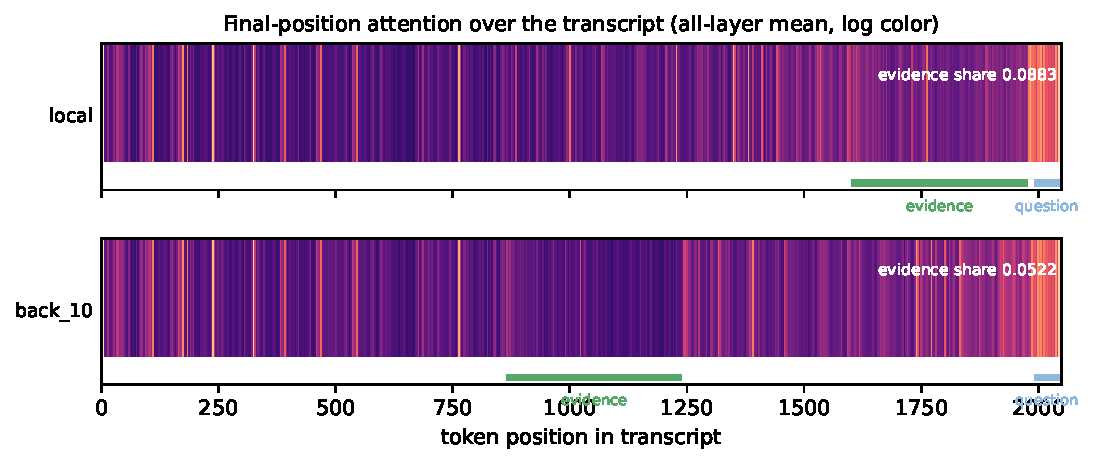
\includegraphics[width=0.98\textwidth]{figures/token_heatmap.pdf}
  \caption{\textbf{Measured final-position attention, token by token} (OLMo-2, all-layer/head
  mean, log-scaled white$\to$orange): windowed excerpts of the same probe's transcript with
  its evidence local vs.\ displaced ten turns back. Solid underline marks the evidence span,
  dashed the current question, and elided stretches are labeled with their token counts. The
  evidence's tint visibly fades when displaced (share $0.088$ vs $0.052$), and the hottest
  tokens in both arms are the chat template's turn delimiters---the concentration whose causal
  role \S\ref{sec:mode} establishes. Built from stored capture rows, not an illustration.}
  \label{fig:token-heatmap}
\end{figure}

\section{Precedent details}
\label{app:precedent-detail}

\begin{figure}[H]
  \centering
  \begin{subfigure}{0.305\textwidth}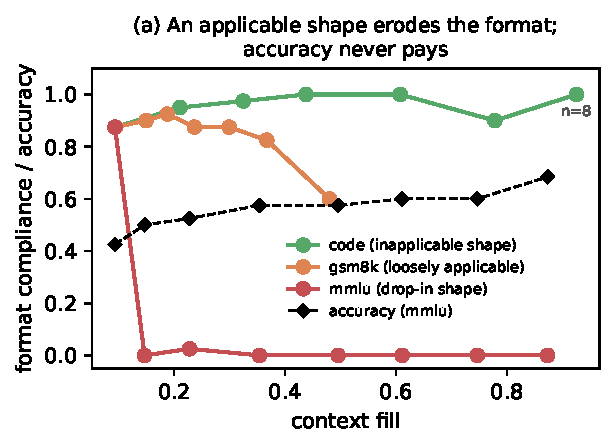
\includegraphics[width=\linewidth]{figures/format_erosion.pdf}\end{subfigure}
  \hfill
  \begin{subfigure}{0.305\textwidth}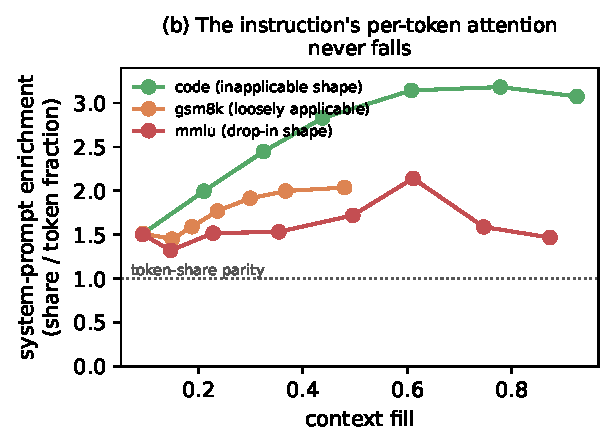
\includegraphics[width=\linewidth]{figures/format_enrichment.pdf}\end{subfigure}
  \hfill
  \begin{subfigure}{0.305\textwidth}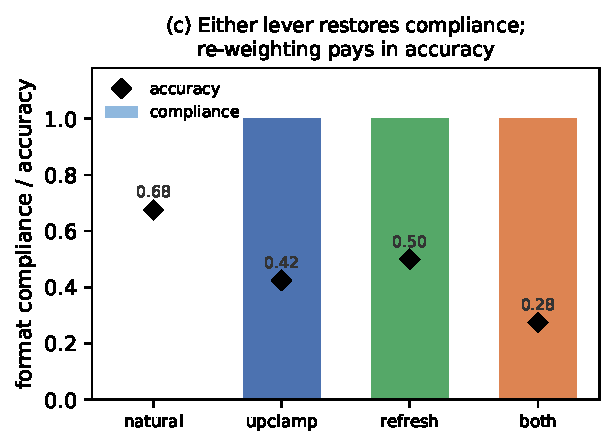
\includegraphics[width=\linewidth]{figures/format_recovery.pdf}\end{subfigure}
  \caption{\textbf{Format erosion is a precedent contest, not attention starvation},
  referenced from \S\ref{sec:precedent}.
  (a) Compliance by fill for three filler streams whose demonstrated answer shapes differ only in
  applicability to the probe. mmlu accuracy (dashed) is unharmed through its total collapse.
  (b) The instruction's per-token enrichment is flat-to-rising in every arm, collapse included.
  (c) At depth 42, clamping the system span's share back up and restating the policy each restore
  compliance fully. Forced mass is paid for in accuracy (zero-sum), restatement is nearly free.}
  \label{fig:erosion}
\end{figure}

\paragraph{The system span's natural trajectory.}
Measured in the clamp experiment's own setup, the system span's share as prior cases accumulate
is $0.166$ (0 cases), $0.081$ (1), $0.060$ (2), $0.037$ (4), $0.028$ (6), $0.021$ (8): an
$8\times$ decline in eight turns from accumulation alone. Clamp ladders must be derived from the
setup they are applied to. A share imported from a different context put two arms above natural,
which were skipped rather than silently clamped upward.

\paragraph{One contrary example overrides the instruction entirely.}
With a single prior case whose answer exhibits the canaries, compliance is $3.00/3$ at every
clamp level down to share $0.021$. With a single bare-letter answer it is $1.00/3$ at every
level including unclamped. $720$ generations per arm, zero variance in reply length ($8$ characters in
one arm, $1$ in the other): the model reproduces the previous assistant turn's format exactly.
Both arms are pinned, one at ceiling because the format is available from the transcript and
one at floor because the contrary example already won, and the clamp has nothing to move. Only the
neutral condition (no assistant turn anywhere) exposes the instruction's causal necessity
reported in \S\ref{sec:precedent}. A ``no demonstration'' arm whose prior turn answers with a
bare letter is not an absence of demonstration but a counter-demonstration.

\paragraph{Exemplar closure.}
At depth 42, closing the demonstrated answer spans' key columns at generation time
(scale $0$, \S\ref{sec:clamp}): all-answer closure $0.000$ compliant, dose-matched partial
closure $0.000$, filler-question closure $0.132$ ($0.100$ in the committed re-run, both
consistent with pure renormalization of the
surviving spans, the system's included), size-matched random-token closure $0.000$. Accuracy
moves within noise. Reading the exemplars at generation time is not what sustains the erosion.
Figure~\ref{fig:closure-dissociation} sets this against the competition rescue: the same
intervention, opposite outcomes.

\begin{figure}[H]
  \centering
  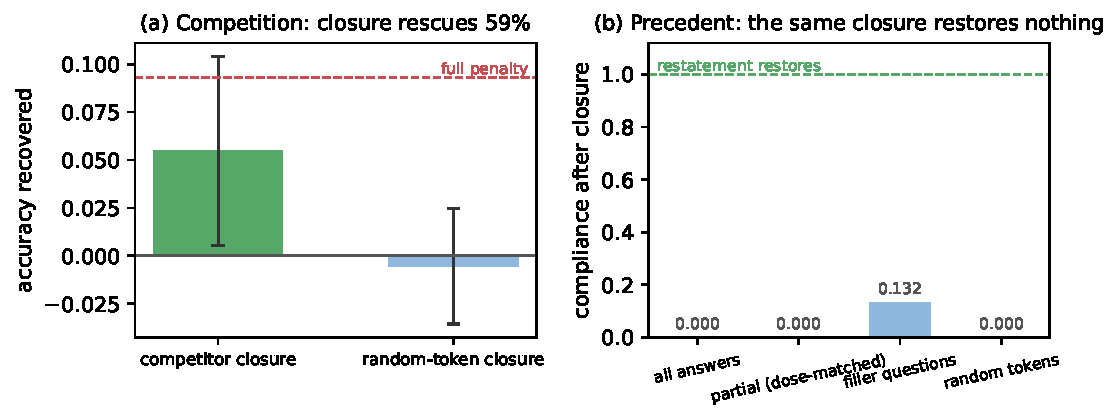
\includegraphics[width=0.9\textwidth]{figures/closure_dissociation.pdf}
  \caption{\textbf{One intervention, opposite outcomes.} The same scale-$0$ generation-time
  closure (a) recovers $56\%$ of the competition penalty (paired $n{=}365$, bars are paired
  accuracy deltas with 95\% CIs, dashed line marks the full in-run penalty), but (b) restores
  no compliance at depth 42 when applied to the demonstrated answer spans ($n{=}40$/arm, every
  closure arm sits at or near the eroded floor while restating the instruction restores
  $1.000$). Competition is generation-time reading. The precedent mode is already in place by
  prefill.}
  \label{fig:closure-dissociation}
\end{figure}

\paragraph{Probes.}
Probe 1 (instruction presence): trained at depth 0 to separate the format system prompt from a
token-length-matched neutral twin. Transfer AUC is $1.000$ at every mmlu depth $0\to42$
(permutation nulls $0.49$--$0.50$, $p{<}0.005$, $n{=}80/76$). The only depth trend is
concentration: mean-over-layers AUC $0.985\to0.791$, peak layer drifting L1--2 $\to$ L11--14.
Probe 2 (upcoming compliance): within gsm8k's mixed cells (same depth, fill, and filler, only
the outcome differs, $n{=}80$), LOO-AUC $0.875$ at stack layer 22 (null $0.485$, $p{<}0.005$),
crossing $0.8$ from layer 18. Vector geometry: the mmlu and gsm8k mode vectors (deep minus
shallow mean differences) have median cosine $+0.746$ across layers---two textually opposite
demonstrated styles shift the residual stream in largely the same direction, with the caveat
that generic deep-context components are common to both.

\paragraph{Steering and erasure.}
Install: the mean-difference vector at stack layer 21, applied at the final prefill position and
every decode step at matched norm, destroys the instructed format in a demonstration-free
context ($0.000$ vs $0.425$ compliant under the norm-matched random control, natural $0.875$),
with replies reproducing the demonstrated registers verbatim. The collateral accuracy cost
($0.175$ vs $0.375$) is consistent with deep-context components inside the mean-difference
vector. A $3\times$ dose breaks generation for real and random alike---controls must be matched
per dose. Erase: four strategies all null with clean controls---the mean-difference direction
projected out at one layer and at eleven (the eleven-layer projection actively harms while its
random control is harmless), and Probe 2's own reader direction projected out at its own layer,
both in-distribution and transferred. Iterative re-probing on the captured states shows the
layer-22 linear code is rank-${\approx}2$ (AUC $0.875\to0.619$ after one fitted projection,
$0.505$ after two), and the erase nulls do not reflect redundancy: the behavioral decision does not
consume the linearly decodable component.

\section{Signature details}
\label{app:signatures-detail}

\begin{figure}[H]
  \centering
  \begin{subfigure}{0.30\textwidth}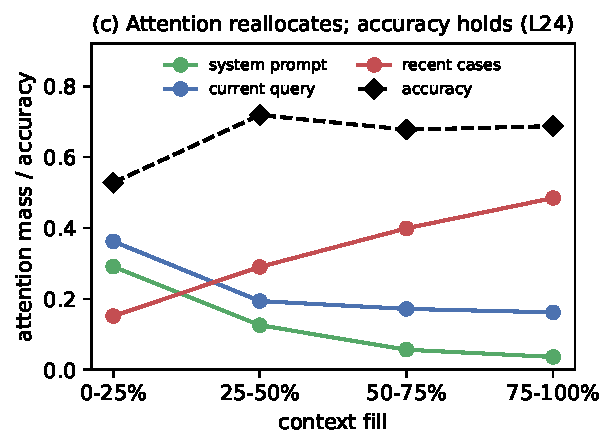
\includegraphics[width=\linewidth]{figures/attention_rot.pdf}\end{subfigure}
  \hfill
  \begin{subfigure}{0.30\textwidth}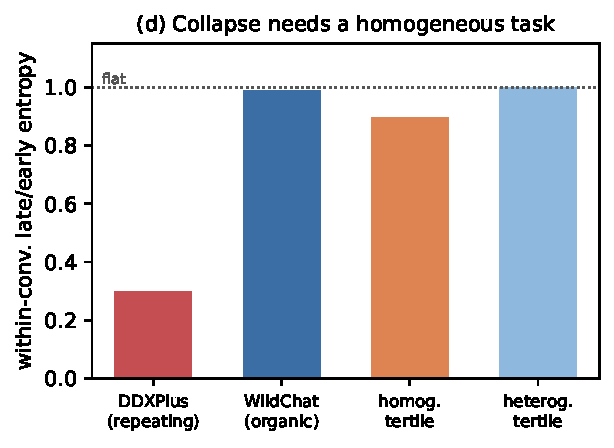
\includegraphics[width=\linewidth]{figures/wildchat_homogeneity.pdf}\end{subfigure}
  \hfill
  \begin{subfigure}{0.30\textwidth}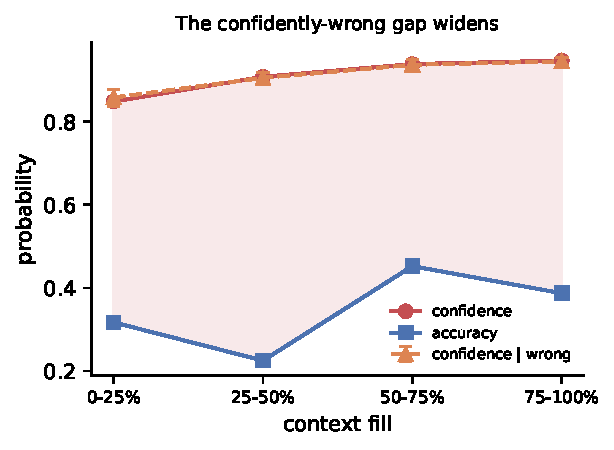
\includegraphics[width=\linewidth]{figures/calibration_gap.pdf}\end{subfigure}
  \caption{\textbf{The signatures track task homogeneity, and the residual hazard is calibration},
  referenced from \S\ref{sec:signatures}.
  (a) Attention reallocates monotonically off the system prompt and current query with fill while
  accuracy holds. (b) The entropy collapse appears only with a homogeneous repeating task, not on
  organic WildChat dialogue, and tracks homogeneity rather than length. (c) Confidence rises with
  fill on wrong answers as much as right, at flat accuracy.}
  \label{fig:signatures}
\end{figure}

\begin{figure}[H]
  \centering
  \begin{subfigure}{0.42\textwidth}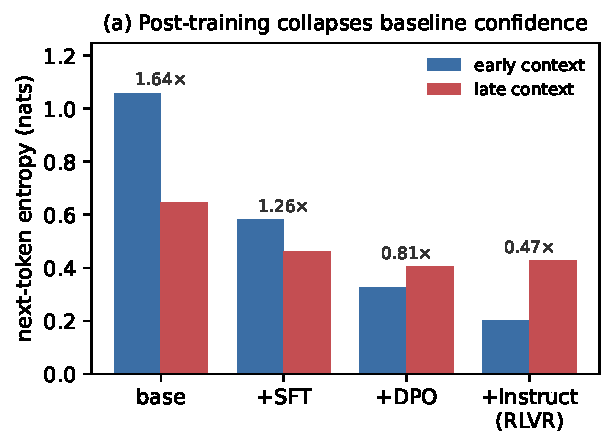
\includegraphics[width=\linewidth]{figures/dose_response.pdf}\end{subfigure}
  \hfill
  \begin{subfigure}{0.42\textwidth}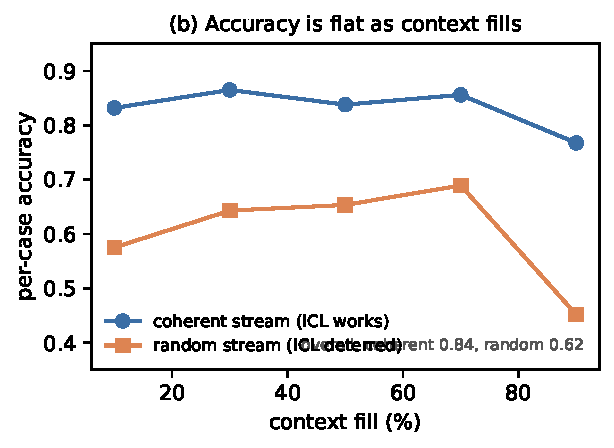
\includegraphics[width=\linewidth]{figures/random_context.pdf}\end{subfigure}
  \caption{\textbf{Signature details.} (a) OLMo-2's post-training chain collapses baseline
  entropy stage by stage. The within-context ratio falls across stages, so alignment
  installs a level shift, not a steeper slope. (b) Accuracy is flat with fill in both the
  coherent and the random-subject stream. The random stream is lower throughout (harder
  subjects), not sloped. Error bars are Wilson 95\% intervals with per-bin $n$ printed. The
  final bins are the smallest ($n{=}31$/$43$) and their intervals overlap the preceding bins',
  so the endpoint movement is not resolved at this $n$.}
  \label{fig:signature-detail}
\end{figure}

\paragraph{Post-training chain.}
Replaying one probe across OLMo-2-7B's base$\to$SFT$\to$DPO$\to$Instruct chain (identical cases
and orders) shows early-context entropy collapsing monotonically, $1.06\to0.58\to0.33\to0.20$,
with the largest single drop at base$\to$SFT (Fig.~\ref{fig:signature-detail}a). The
``collapses as context fills'' framing is mostly a base-model ICL effect plus a floor: the
within-context ratio falls across stages ($1.64\to0.47$), because aligned models start
near an entropy floor.

\paragraph{WildChat.}
Median within-conversation $\mathrm{corr}(\text{entropy},\text{depth})$ is $-0.02$ on organic
dialogue ($150$ conversations, $2{,}039$ boundaries). The homogeneity partition is a separate
$400$-conversation run: tertiles of inter-turn TF-IDF similarity give late/early ratios $0.897$
(homogeneous) vs $1.001$ (heterogeneous), $n{=}134$ per tertile. Homogeneity correlates with
the entropy slope (Pearson $-0.141$ at $p{=}0.005$, Spearman $-0.103$ at $p{=}0.039$, partial
$r=-0.151$ controlling for length) and with conversation length ($+0.155$: homogeneous
conversations are longer, and length works against the effect). The tertile medians are reported
without intervals.

\paragraph{A proposed mechanism that fails causally.}
Clamping the boundary-detector SAE feature (Gemma Scope F90871,
\citealp{lieberum2024gemmascope}) back to its clean level on held-out fatigued cases moves
entropy the wrong way ($0.442\to0.465$ vs clean $0.293$), leaves accuracy flat, and a
random feature of similar magnitude perturbs entropy at least as much.

\paragraph{Attention and errors point the other way.}
Conditioning on fill, the cases OLMo-2 answers wrong have higher current-query
attention than the ones it gets right (pooled $\Delta=+0.045$ $[-0.003,+0.097]$, $n{=}115$). The
interval touches zero, but the sign is positive in every fill bin and at every probed layer, an
observational pattern rather than an established one. Errors
co-occur with fixating on the query while correct answers spread attention onto the
accumulated cases---the per-case fingerprint of the in-context learning that keeps accuracy up,
with the ``rot'' and the within-context predictor of a correct answer pointing in opposite
directions.

\section{Cross-family replication: Qwen2.5-7B-Instruct}
\label{app:qwen}

The causal program was re-run on Qwen2.5-7B-Instruct (seed 42, $4$k window, same drivers,
panel
constructions, and drop rules as the committed OLMo runs). The window matches the OLMo runs,
and the cross-family contrasts below, the competition divergence included, are not window
effects. Share readouts are all-layer pooled
except the distance sweep's, which is layer-24-indexed like OLMo's.
Table~\ref{tab:crossfamily} is the summary; the per-experiment detail follows it. Nine of the
paper's claims reproduce, two reproduce in part, and the three that make up the competition
result do not.

\begin{table}[H]
  \centering\small
  \caption{\textbf{Every claim, in both families.} Accuracy contrasts in percentage points,
  compliance as a fraction. ``partial'' marks a claim that holds in direction but not in
  degree; ``inverted'' marks a measurement whose sign differs with disjoint intervals. Two
  rows quote the statistic each run recorded rather than a common one: the accumulation row is
  OLMo's fill correlation against Qwen's fill slope (both over random and coherent streams,
  all n.s.), and the system-clamp row is OLMo's compliance collapse against the share at which
  each of Qwen's two canary duties fails. Both families run at seed 42 in a $4$k window on the
  same panels, so no row is a window effect.}
  \label{tab:crossfamily}
  \setlength{\tabcolsep}{4pt}
  \begin{tabular}{@{}l l l l@{}}
    \toprule
    claim & OLMo-2-7B & Qwen2.5-7B & holds\\
    \midrule
    accumulation costs no accuracy & $r=-0.02$, $+0.03$ & slope $-0.06$, $-0.09$ & yes\\
    displacement ladder is monotone & $0.464\to0.276$ & $0.630\to0.469$ & yes\\
    \quad and saturates by $k{\approx}10$ & $0.250$ then $0.276$ & $0.505$ then $0.469$ & partial\\
    mass removal reproduces the gap & $91\%$ & $107\%$ & yes\\
    the dose-response is graded & $0.473\to0.275$ & $0.667\to0.380$ & yes\\
    \quad with no threshold in it & max step $0.053$ & no knee & yes\\
    clamping the system span kills compliance & $0.99\to0.03$ & at shares $0.12$, $0.09$ & yes\\
    erosion tracks applicability & $1.00/0.60/0.00$ & $1.00/1.00/0.00$ & yes\\
    \quad and is total & $0.875\to0.000$ & \texttt{ANSWER:} only & partial\\
    restating the instruction reverses it & $1.000$ & $1.000$ & yes\\
    re-weighting it reverses it & $1.000$ & $0.733$ & partial\\
    the demonstrated answers are read & $+1.28$ & $+0.87$ to $+1.49$ & yes\\
    \midrule
    near-duplicate context costs accuracy & $+8.5$ & $+3.0$, n.s. & no\\
    closing the competitors rescues it & $+6.0$ ($56\%$) & $+1.9$, n.s. & no\\
    the evidence's share under \texttt{near\_dup} & $+0.0003$, n.s. & $+0.0071$ & inverted\\
    \bottomrule
  \end{tabular}
\end{table}

\noindent Two qualifications the table cannot carry. The cross-family
difference-in-differences on competition (OLMo's paired penalty minus Qwen's) is $+5.5$ points
$[-1.5,+12.5]$, suggestive and not significant, so the divergence rests on the closure null and
the inverted share rather than on a direct interaction test. And Qwen's low-competition arms
sit ${\approx}10$ points above its own \texttt{local} arm, because same-task context practices
the probe's task where MMLU filler does not; cross-family comparisons of arm levels inherit
that practice benefit, and only within-family gaps are interpreted.

\begin{table}[H]
  \centering\small
  \caption{\textbf{Counterfactual patching of the format-instruction state} (Qwen2.5-7B,
  \texttt{code} cell), referenced from \S\ref{sec:mode}. Full-transcript row $n{=}39$,
  bisection rows $n{=}23$.
  $\Delta\Delta = \Delta\ell_{\mathrm{patch}} - \Delta\ell_{\mathrm{self}}$: the shift of the
  instructed-formats log-probability contrast $\Delta\ell$ against a self-patch baseline.}
  \label{tab:patch}
  \setlength{\tabcolsep}{5pt}
  \begin{tabular}{lcc}
    \toprule
    patched positions & $\Delta\Delta$ & share of full\\
    \midrule
    full context, all layers & $-2.488$ & $100\%$\\
    template glue (\texttt{im\_end}/\texttt{im\_start}) & $-1.540$ & $62\%$\\
    assistant turns & $-0.287$ & $12\%$\\
    user turns & $+0.165$ & ---\\
    last $1$/$2$/$4$ turns & $\leq|0.075|$ & ${\sim}0$\\
    size-matched random positions & $+0.016$ & ---\\
    template glue $\times$ layers $7$--$13$ & $-1.051$ & $42\%$\\
    \bottomrule
  \end{tabular}
\end{table}

\begin{figure}[H]
  \centering
  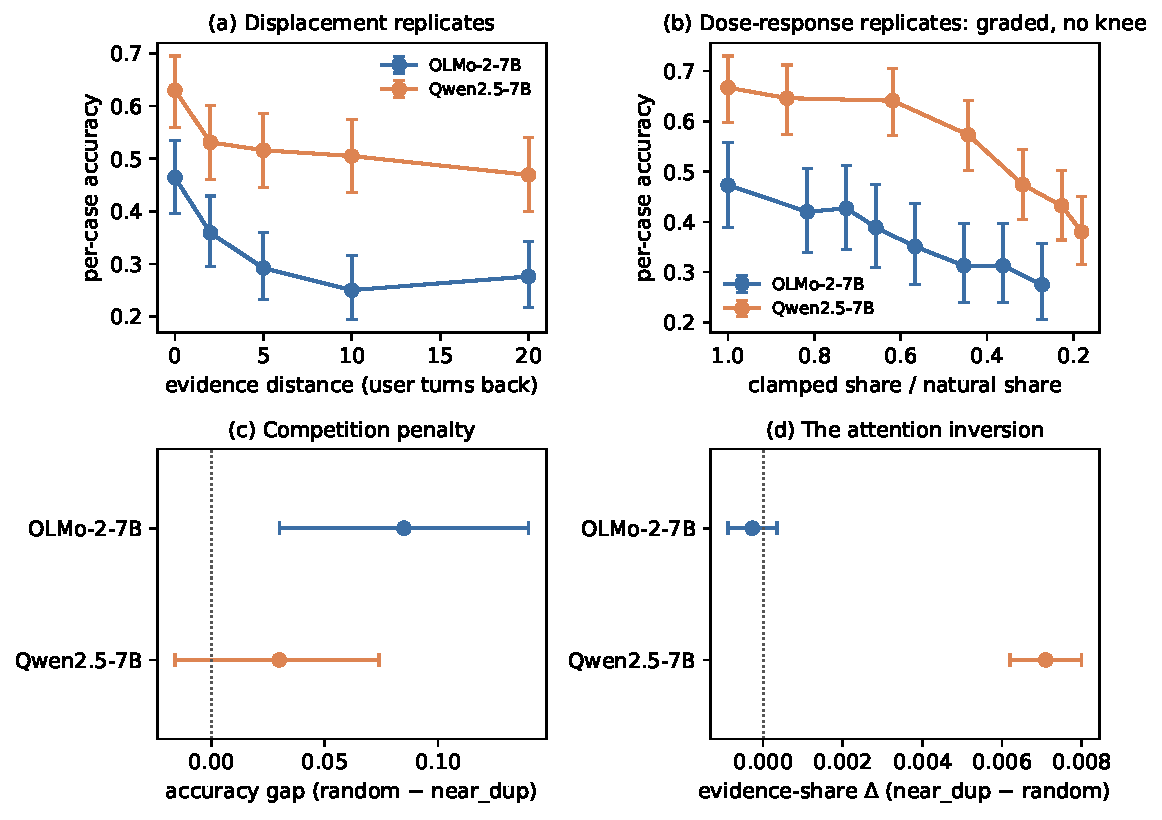
\includegraphics[width=0.92\textwidth]{figures/qwen_replication.pdf}
  \caption{\textbf{The causal program replicates on Qwen2.5-7B, except competition.}
  (a) The distance ladder at matched fill ($n{=}192$/arm in both families).
  (b) The share$\to$accuracy dose-response, $x$ as a fraction of each family's natural share
  (OLMo layer-24-indexed with common subset $n{=}131$, Qwen all-layer with $n{=}181$--$192$): graded
  with no knee in both. (c) The competition contrast is significant on OLMo, not detected on
  Qwen. (d) The evidence's attention under near-duplicate context: flat on OLMo, rising
  on Qwen, with disjoint intervals---the family divergence. Whiskers in (a,\,b) are per-point
  Wilson 95\% intervals. Panels (c,\,d) show the paired bootstrap CIs quoted in the text.}
  \label{fig:qwen-replication}
\end{figure}

\paragraph{Displacement.}
The ladder reproduces fully monotone: $0.630 \to 0.531 \to 0.516 \to 0.505 \to 0.469$
($n{=}192$ per arm, $0$ overflow skips), every paired gap significant
(\texttt{back\_2} $+9.9$ points $[+5.2,+14.6]$ through \texttt{back\_20} $+16.1$
$[+9.4,+22.9]$). In the joint fit distance carries the coefficient ($-0.0061$
$[-0.0102,-0.0016]$) and fill is significant only with the opposite sign
($+0.330$)---byte-identical fill across arms cannot carry the ladder. Qwen answers with a bare
letter ($0.0\%$ unparsed), and the ladder needs no parsed-only robustness arm: the truncation
caveat attached to the OLMo ladder does not arise on this family.

\paragraph{Mass sufficiency and dose-response.}
Clamping \texttt{local} evidence to \texttt{back\_20}'s share reproduces $107\%$ of the
distance gap (mass alone $+16.7$ points $[+10.4,+22.9]$ against a gap of $+15.6$
$[+8.9,+22.4]$). The clamped arm is indistinguishable from \texttt{back\_20} (residual
$-1.0$ points $[-5.7,+3.7]$). The share sweep is graded with no knee, still falling below the
deepest natural share ($0.667$ at natural to $0.380$ at share $0.0070$), and its causal slope,
$+10.4$ $[+7.6,+13.6]$ accuracy per unit share, matches the observational
fit of correctness on share ($+10.7$ $[+3.5,+17.6]$) from a separate design (the
observational fit is on the distance sweep's layer-24 shares, the causal slope on all-layer
shares, and the agreement is suggestive rather than unit-exact).

\paragraph{Accumulation and the system clamp.}
The random-subject stream is flat across its $4$k window (fill slope $-0.057$ $[-0.238,+0.135]$, with the coherent stream at $-0.090$, also n.s.), and the adherence canaries do not decay. Clamping the system
span's share collapses compliance at graded dose with a duty ordering, the reply's
separately-graded obligations failing one at a time: reply-prefix canary
first (at share $0.12$), suffix next ($0.09$), the forbidden-phrase rule never
(Fig.~\ref{fig:qwen-clamp}). Meanwhile accuracy rises under the clamp ($-0.09$
$[-0.16,-0.03]$ at the deepest level), the zero-sum reallocation that was directionally present
but n.s.\ on OLMo.

\begin{figure}[H]
  \centering
  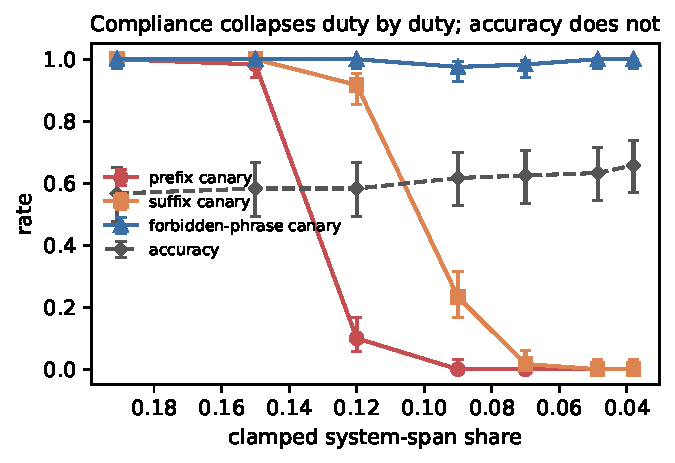
\includegraphics[width=0.55\textwidth]{figures/qwen_system_clamp.pdf}
  \caption{\textbf{Qwen's system clamp collapses compliance duty by duty.} Neutral-context
  clamp ($n{=}120$/level): the reply-prefix canary dies between shares $0.15$ and $0.12$, the
  suffix between $0.12$ and $0.09$, the forbidden-phrase rule never. Accuracy is flat-to-rising
  throughout. Whiskers are Wilson 95\% intervals.}
  \label{fig:qwen-clamp}
\end{figure}

\paragraph{Precedent.}
The applicability ordering confirms: \texttt{mmlu} compliance $1.000 \to 0.000$ within three
filler turns while \texttt{gsm8k} and \texttt{code} hold $1.000$ through fill $0.84$--$0.92$,
accuracy flat throughout (overflow skips thin \texttt{code} to $n{=}17$ at its deepest fill). The demonstrated-answer reading signature reproduces
(answer-over-question enrichment $+0.87$ to $+1.49$ in \texttt{mmlu} at every depth, negative
in \texttt{code}---the erosion ordering). Two results differ. Erosion is staged rather than
total: the \texttt{ANSWER:} marker dies immediately while the \texttt{SUPPORTING} duty
survives to mid-depth, the same duty ordering the clamp produces causally. Restatement beats
re-weighting: at depth 42, refreshing the instruction restores $1.000$ while upclamping the
system span restores only $0.733$ (both at no accuracy cost). One dissociation does not carry
over: Qwen's compliant arms sit at or above the share where its own clamp collapses the prefix
duty and its eroding arm below it, and Qwen's erosion arms do not by themselves exclude a mass
account the way OLMo's \texttt{code} arm (full compliance at half \texttt{mmlu}'s share) did.

\paragraph{Competition: the family divergence.}
The three competition rows of Table~\ref{tab:crossfamily} are one result: on the same
$n{=}365$ panel the penalty is not detected, the competitor closure that rescues OLMo does
nothing, and the evidence's share moves the other way with disjoint intervals. Qwen defends
the evidence under confusability rather than merely not paying for it.

A masked-channel account is available. By Qwen's own dose-response slope the share it gains
under \texttt{near\_dup} should be worth ${\approx}7$ points of accuracy, yet the arm
underperforms that prediction by ${\approx}10$ points, close to OLMo's penalty. On that
reading Qwen pays the same cost and hides it behind a compensating attention gain. The
account stacks coefficients estimated in different designs, and we mark it interpretive. What
the closure null does establish either way is the channel: whatever the shortfall is, it is
not carried by the competitor-mention tokens that carry OLMo's cost.

\subsection{Counterfactual instruction patching and the carrier bisection}
\label{app:patching}

This is the instrument behind \S\ref{sec:mode}'s token-level localization.

\paragraph{The instrument.}
Build two transcripts that are identical in filler and probe and differ only in the system
instruction: $T_A$ carries an \texttt{ANSWER:} prefix format, $T_B$ a one-line JSON format.
Fix one reply in each format, $y_A$ and $y_B$, and score a transcript by how much it prefers
one over the other under teacher forcing,
\[
  \Delta\ell(T) \;=\; \log P(y_A \mid T) \;-\; \log P(y_B \mid T).
\]
$\Delta\ell$ is large when the model is disposed to answer in format $A$ and small when it is
disposed to answer in format $B$, so it reads out the disposition \S\ref{sec:mode} calls the
mode without requiring the model to emit anything.

A difference of log-probabilities between two fixed continuations is the readout
\citet{wang2023ioi} established for circuit-level patching, and \citet{zhang2024patching}
survey it against the probability- and accuracy-based alternatives. Two of its properties
decide the choice here. It is linear in the logits, so a patch that moves the contrast by a
given amount moves it by that amount wherever the model sits on its confidence curve, which a
probability readout does not do once either format saturates. And it cancels any shift common
to both continuations: the deep \texttt{code} cell runs with the system span closed, which
depresses the likelihood of every well-formed reply at once, and a metric scoring one format
alone would register that as an effect. Only the contrast between the two survives it.

Now move the state. Write $h_P(T)$ for the hidden states captured from $T$ at a set of token
positions $P$, and $T \leftarrow h$ for a forward pass on $T$ whose prefill activations at
those positions are overwritten with $h$. The counterfactual patch transplants the donor's
states into the recipient at $P$; everything else about the recipient is untouched. This is
activation patching in the causal-mediation form introduced by \citet{vig2020mediation} and
used for factual recall by \citet{meng2022rome}, with the instruction rather than a fact as
the mediated variable. All cells
run in the A$\to$B direction, $A$ donating and $B$ receiving, in the deep \texttt{code} cell
at depth 15 with the system span closed. The full-transcript patch is the stage-1 run at
$n{=}39$ and the bisection cells are $n{=}23$ after one overflow skip.

\paragraph{The estimand.}
The quantity in Table~\ref{tab:patch} is the interaction contrast
\[
  \Delta\Delta(P) \;=\; \underbrace{\Delta\ell\big(T_B \leftarrow h_P(T_A)\big)}_{\text{patched with the donor's states}}
  \;-\;
  \underbrace{\Delta\ell\big(T_B \leftarrow h_P(T_B)\big)}_{\text{patched with its own states}},
\]
a difference-in-differences in which both arms undergo the identical capture-and-splice
procedure at the identical positions, and the only thing that differs is whose states were
spliced in. A large $|\Delta\Delta(P)|$ means the positions in $P$ carry the format
instruction's effect; a $\Delta\Delta(P)$ near zero means they do not. The ``share of full''
column normalizes each cell against the whole context,
$\Delta\Delta(P)\,/\,\Delta\Delta(\text{all positions})$.

The baseline is the self-patch rather than an unpatched run, and that choice is what makes the
measurement work. Donor states are captured with the system span open, while a pure run forms
its states with that span closed, so $\Delta\ell(T_B)$ and
$\Delta\ell(T_B \leftarrow h_P(T_B))$ differ by a capture-openness term that has nothing to do
with donor identity. In preflight an unpatched baseline confounded exactly that term with the
effect of interest, and the unrelated-fact control moved as much as the counterfactual patch;
against the self-patch baseline the same control is null. Identification then needs only
additivity, that capture-openness shifts both arms' contrasts by the same amount, which is
what sharing one procedure across arms is designed to buy.

\paragraph{Where the state lives.}
The full-transcript patch moves the contrast by $\Delta\Delta = -2.488$. Bisecting by position,
every content subset is near null. The context's assistant turns carry $-0.287$, its
user turns $+0.165$, and its last $1/2/4$ turns at most $|0.075|$. The chat template's turn
delimiters alone carry $\mathbf{-1.540}$, $62\%$ of the full effect, against a size-matched
random-position control of $+0.016$. Those delimiters contain no instruction text and no
demonstrated answer. Bisecting by depth instead, layer-block patches at all positions give
$-1.16$ (layers $0$--$6$), $-1.59$ ($7$--$13$), $-0.45$ ($14$--$20$), and $-0.11$
($21$--$27$). The blocks overlap in what they carry, so their sum exceeds the full effect.
Crossing the two, glue positions restricted to layers $7$--$13$ still carry $-1.051$ ($42\%$)
while touching no content token and no layer above $13$. Earlier waves that searched
inside the turns, by role and by recency, came back null: the state rides
between the turns rather than in them.

\paragraph{Specificity control.}
The control throughout is an unrelated-fact patch, the same instruction with one irrelevant
clause changed, token-matched. It stays at $\le|0.11|$ in every quoted cell except two, and
both of those have counterfactual effects that are themselves near null: the last-$2$-turns
cell at $+0.26$ and the random-position cell at $-0.11$.

\paragraph{Two caveats on the readout.}
Under closure Qwen emits no canonical format in free generation, in none of the $90$ graded
replies across both patch arms. The estimand lives in the teacher-forced contrast
alone, with no generation-level corroboration in this cell. Closure also drops the recipient's
system-span identity out, which makes the two patch directions exact mirror images
($\Delta\Delta_{B\to A}=-\Delta\Delta_{A\to B}$), so the quoted direction is the one
independent measurement. The full effect is also sign-inverted relative to the donor's
instruction, in that A-donor states depress the A-format productions. The localization claim
does not depend on that. The bisection asks where the state travels, not which way it
pushes.

\end{document}
